\documentclass[12pt, twoside]{article}
\usepackage{style}
\setabbreviationstyle[acronym]{long-short}
\newacronym{LLM}{LLM}{large language model}
\newacronym{ENOE}{ENOE}{Encuesta Nacional de Ocupación y Empleo}
\newacronym{DID}{DiD}{Differences in Differences}
\newacronym{SINCO}{SINCO}{Sistema Nacional de Clasificación de Ocupaciones }
\newacronym{AI}{AI}{Artificial Intelligence}
\newacronym{INEGI}{INEGI}{Instituto Nacional de Estadística y Geografía}
\newacronym{ETOE}{ETOE}{Encuesta Telefónica de Ocupación y Empleo 2020}
\newacronym{ENOEN}{ENOEN}{Encuesta Nacional de Ocupación y Empleo Nueva Edición}
% \newacronym{internal-name}{displayed-name}{long-name}
% \makeglossaries   %pegar el glosario de palabras
% \acrfull{}                                                             
% \acrlong{}
% \acrshort{}

\title{How do mexican labor markets adjust to ChatGPT on the short term?\thanks{I thank XXXX. I take full responsibility for any remaining errors in this work.}}
\author{Maximiliano Ochoa Trancoso\thanks{Student of Undergrad Program in Economics at El Colegio de México. Email: \href{mailto:mochoat@colmex.mx}{mochoat@colmex.mx}} \\ [-1pt]{\normalsize \textit{El Colegio de México}} \\}

\date{Fall 2026}


\begin{document}

\begin{singlespace}
    \maketitle
    \begin{abstract}
        Abstract
    \end{abstract}

    \keywords{GPT, DiD, worker flows, employment}
\end{singlespace}
\newpage
\tableofcontents

\newpage
\section{Introduction}

ChatGPT was launched by OpenAI november 3oth of 2022. It is powered by GPT-3. A \glsxtrfull{LLM} trained wiht massive data across WebText2. This includes websites, books, articles and toher types of text based information. It is cappable of analyzing stadistical relationships between words and phrases. This way, the model is extraordinarily efficient in tasks such as generating, summarizing and translating text in a coherent way. \citep{RAY2023121}

Even though many of the capabilities of ChatGPT were already maneagable with GPT-2 since 2019, the main different aspect of GPT-3 which I will be expLoiting is its universal accessibility. In november 2022 the launch of ChatGPT stormed into society's psyche via public use with no payment requiered, an easy interface simple enough to only input a question and an easygoing nature capable of running on most devices. In january 2023, 2 months after its launch, the agent reached around 100 million users. \footnote{\cite{paris2023chatgpt}} 

The fast technological shift due to \glsxtrshort{LLM}'s has sparked a heated debate as enterprises and governments adapt to the new paradigm. This debate is central to the thesis I present as one of the main points of disagreement is the effect that \glsxtrshort{LLM}'s have on the labor market.

In economic theory the effects are ambiguous. On one hand, \glsxtrshort{LLM}'s can be mere complements by enhancing worker's performance. ***** on the other hand, it completely subsitutes out workers in certain fields. \citep{hui2024short} Thus it is of great importance to the mexican market to analyze the function an \glsxtrshort{LLM}, such as ChatGPT, has on tasks in order to understand potential wage differentials and job transitions. 

Previous literature has found that adoption of other similar tecnhologies such as computers can worsen wage inequality and affect negatively employment levels. \citep{krueger} \citep{katz} \citep{autor2003} Moreover, the mexican context is a particular case in which its persistent informality can weaken or strengthen these effects. 

With the launch of ChatGPT as an exogeonous event I use the rotative panel \glsxtrfull{ENOE} and estimate the emplyment and wage effects in the mexican labor market. My main specification is a \glsxtrfull{DID} and it is inspired by \cite{hui2024short}'s model. I classify exposed tasks and construct an occupation\footnote{I construct an individual index for all occupations in \glsxtrshort{ENOE} according to \glsxtrfull{SINCO}} specific index relying on methodology by \cite{martinez2024risk} and \cite{eloundou2023gptsgptsearlylook}.

I provide the first estimates for labour and wage impacts due to the launch of ChatGPT in Mexico. These reults reveal XXXX.


%% Añadir analisis de compsicion industrial 

\section{Related literature}

Technological change is a constant force of nature that has been around for thousands of years. The still ongoing debate referring to the effect on wages and employment has been parallel to almost every major techonlogical change. Recently, the introduction of \glsxtrfull{AI} and \glsxtrfull{LLM}'s reignited this debate since the capabilities shown by these technologies are extraordinary in the sense that they are capable of automating certain non routine cognitive tasks.The ambiguity of the effect on employment and wages that recent and historical studies have found inspires the scope of my main research question. How does the release of ChatGPT affect employment, wages and informality in Mexico? In order to understand this question I review literature surrounding technological change and its role in task automation, wages and employment. Second, I take a look at recent studies on the effect of \glsxtrshort{LLM}'s on employment and wages in an effort to understand the current state of the debate even though the literature is still new. Finally, the setting of my research question revolves around Mexico. Because of this, an important strand of literature I explore is the one that studies the dynamics of technological change in developing countries, escpecially Latin America.

Back in the 90's, there was a strand of literature trying to make sense of the increasing wage premium of skilled workers and technological unemployment. First, \cite{katz1992changes} develop a supply and demand model in an effort to understand the rising wage inequality and wage struture in the US. The authors find that the rising supply and demand for skilled workers shifted the college wage premium. They also attribute the changing wage structure to compositional shifts in relative labor demand within sectors due to skill biased technological change.  Then, \cite{krueger} examines employees who use a computer at work in an empirical framework. The author's estimates suggest a 10 to 15\% higher wage rate and above average wage growth in occupations with growing computer use. Meanwhile, \cite{cox}'s approach shows a temporary unemployment effect due to technological change. Throughout the decade some critics were issued \citep{dinardo} and by the end of the decade and the following years, \cite{katz1999} \& \cite{goldin2007} solidify the analysis by understanding the link between market forces and market institutions. The conclusion puts computers and fluctuations in the supply of more educated workers as the main suspects behind the skill wage differential.

What followed was a way to understand the mechanisms behind the skill premium after a technological change. \cite{murnane} investigate how the demand shift favored college labor. They come out with a framework capable of analyzing how computers change the demand of tasks on the job. They find that across industries, occupations and education groups, computers reduce routine manual and routine cognitive tasks and increase non routine cognitive tasks in labor input. Using this framework, research revolved around \textit{job polarization}. A phenomenon in which jobs are polarized into high wage and low wage, pushing out middle skill jobs  \citep{goos,autorkatzkearney}. The phenomenon is then linked with the growth of low skill jobs and falling costs of automating routine job tasks \citep{goos2014,autor2014}. Trying to understand the forces behind job polarization, \cite{acemoglu2018} explains two effects relating to the role of automation in task creation and destruction. The first one of these is a \textit{displacement effect} in which automation destroys tasks previously performed by labor. The second one is a \textit{productivity effect} that creates new tasks which are not yet able to be automated. These opposing effects result in ambiguous effects on wages and employment. The importance behind this framework relies on its capacity to explain how tasks exposed to automation are key in explaining the final outcome relating wages and employment. Tasks are not randomly exposed to automation. A technological change may involve destruction of tasks mostly performed by low or high skill workers and many authors exhibit concerns referring to wage inequality \citep{murnane,goldin2007,goos,goos2014,autor2014,brynjolfsson2014second,stiglitz2017artificial}. Because of the great importance behind this framework, I use it to disentangle and interpret the mechanisms behind my main results.

Branching out from this literature there is a new set of studies analyzing \glsxtrshort{AI}. The main difference this technology has showed is that \glsxtrshort{LLM}'s are capable of automating certain non routine cognitive tasks \citep{eloundou2023gptsgptsearlylook}. Although this difference shifts every notion of automated tasks we preiously had with computers, the framework established by \cite{acemoglu2018} is able to explain many details regarding the new technological paradigm. \cite{eloundou2023gptsgptsearlylook} develop an exposure index to \glsxtrfull{AI} by classifying 19,265 tasks from O*NET\footnote{A database that enlists occupation specific task statements in order to describe what a worker does in their respective occupation} with human tests and ChatGPT. The results point to 15\% of all tasks in the United States being completed much faster with the same quality when exposed to an \glsxtrshort{LLM}. This estimate increases to between 47\% and 65\% if additonal tools are considered to work alongisde the \glsxtrshort{LLM}. These findings point to a low share of tasks that can be fully automated. Moreover, \cite{eloundou2023gptsgptsearlylook} highlight higher income jobs facing higher exposure. The finding is further solidified by \cite{Felten2023OccupationalHI}, who characterizes exposed occupations as highly educated, highly paid and white collar.

Several empirical and behavioural papers have followed \cite{eloundou2023gptsgptsearlylook} trying to determine the ambiguous effect on wages and employment, and the extent to which \glsxtrshort{LLM}'s create new tasks for a given occupation. First, \cite{noy} provide experimental evidence highlighting that ChatGPT benefits low skill workers by restructuring tasks and compressing the productivity distribution. \cite{hui2024short} use \glsxtrshort{DID} to estimate the effect of ChatGPT's release and other \glsxtrshort{LLM}'s on wages and employment for a large digital platform for freelancers. Their results suggest a fall in employment and wages for writers, designers and artists; especially those who are top rated. This last result may point to the possibility of shortening the wage gap between workers in the same exposed field. \cite{Dang} use the Current Population Survey (CPS) and a Synthetic \glsxtrshort{DID} and estimate the impact of ChatGPT's release on the united states's labour market. They find opposite results to \cite{hui2024short} in the form of a modest increase in wages for the exposed group and relatively no changes in unemployment for all population. \cite{humlum} rejects the idea that ChatGPT has a disruptive effect on the danish labor market and finds no effects on wages or employment. However, the authors do point out a major reorganization of tasks in exposed occupations. In summary, the literature related to \glsxtrshort{LLM} and its effects on the labor market does not follow a clear pattern.

Finally, the developing country evidence highlights certain dynamics developing countries do not face. Phenomenons such as informality complicate certain aspects of potential effects of \glsxtrshort{LLM}. Moreover, \cite{neto} nuances the job polarization narrative in developed economies for developing economies including Latin America. The authors find a moderated job polarization that is explained by limited technology adoption, structural change and changes in the global value chains. On the other hand, exposure to \glsxtrshort{AI} shows a clear pattern in Latin America.  Higher exposure is concentrated among women, urban, educated and formal workers \citep{azuara,worldbank,martinez2024risk}. This implies a major concern for labor inequality in the region in the following years. Specifically, \cite{martinez2024risk} adapt methodology by \cite{eloundou2023gptsgptsearlylook} and replicate their exposure index for the mexican context with \glsxtrfull{SINCO}\footnote{ \glsxtrshort{SINCO} enlists around 3,000 tasks for 468 occupations}. I use their measures in order to characterize occupations potentially exposed across several groups. The effort to estimate the ambiguous effect on employment and wages is uncharted territory in Mexico. My analysis is the first empirical approach to labor market outcomes in Mexico and one of the first for developing economies.





\section{Data, treatment and outcomes}

In order to conduct my analysis, I use data from \glsxtrfull{ENOE} conducted by \glsxtrfull{INEGI}. Since 2005, this survey reports quarterly data related to labour statistics for the Mexican population aged 15 and older. It is a rotating panel that follows 5 subsamples for up to five quarters with a probabilistic design.

Because of the COVID-19 pandemic, \glsxtrshort{INEGI} was not able to conduct its regular survey during the second quarter of 2020. This led to the construction of a new temporary survey (\glsxtrfull{ETOE}). The discontinuity resulted in the creation of \glsxtrfull{ENOEN}, a version of \glsxtrshort{ENOE} featuring an updated survey design and a mixture of face-to-face and telephone interviews, implemented from the third quarter of 2020 through the fourth quarter of 2022. From the first quarter of 2023 onwards, \glsxtrshort{INEGI} resumed the regular \glsxtrshort{ENOE} while maintaining comparability with \glsxtrshort{ENOEN}. To ensure consistency over time within the survey framework, I limit the sample to observations from the third quarter of 2020 through the second quarter of 2026 . Following standard \glsxtrshort{ENOE} procedures, I restrict the sample to individuals with completed interviews, valid residence status and aged 18 to 64 years old.

The \glsxtrshort{ENOE} data does not allow to follow individuals over long periods of time. Therefore, for my estimations, I aggregate the individual level data to the occupation level. The main advantage related to this data structure is that it allows me to follow cells for several quarters while also being able to measure the mass of employed people in each occupation across time. Occupations are identified using \glsxtrfull{SINCO} codes present in both \glsxtrshort{ENOEN} and \glsxtrshort{ENOE}\footnote{The \glsxtrshort{ENOE} survey uses \glsxtrshort{SINCO} codes from the 2011 methodology until the second quarter of 2021. From the third quarter of 2021 onwards the survey uses the 2019 \glsxtrshort{SINCO} classification. Because of this I harmonize codes using the official \glsxtrshort{INEGI} cross walk table.}. For each occupation $j$ in quarter $t$, the outcomes variables are defined as the weighted average outcome among workers employed in occupation $j$\footnote{Weights are specifically the \glsxtrshort{ENOE} expansion factors. This way each mean is representative of the number of workers in that occupation}. The resulting dataset is a pseudo-panel following 422 occupations\footnote{The original count is of 483 codes. However, I exclude code 9999 (non classified occupations) and restrict my analysis to occupations that have at least one worker observation across all quarters.} which represents roughly 52.6 million workers based on the last quarter of 2022. The range of weighted observations goes from 46.6 to 54 million, and raw observations go from 110 thousand to 184 thousand. This huge gap is caused by the first four quarters in my sample. Because of Covid, a large number of intervies were not ablet o be finished in person so the count drop spikes the standard errors in the first few quarters. This poses no threat to vailidity since further quarter have more stable counts and the drop is further from the treatment period.

The outcomes of interest for my analysis are the share of informal workers, the number of employed people and average wages in occupation $j$. The share of informal workers include workers employed in the informal sector as well as workers whose employment relationship lacks access to the legal and institutional protections associated with formal employment. The number of employed people come directly from the number of workers in occupation $j$ at quarter $t$.

Wages are monthly earnings in nominal pesos. However, a problem with \glsxtrshort{ENOE} is that a non random share of paid employed workers report zero hourly income despite working a positive number of hours and reporting an occupation. \cite{imput}
I treat these as missing and impute them with a predictive mean matching (PMM) method develoepdd by \cite{conasami2023imputacion}. I split workers who need imputed wages into those that did not gave an answer to a minimum wage bracket and those who did. Each group of workers is then imputed a wage using two different models. In both models, donors are workers who reported an exact amount. Then, for model 1, regresses income on worker characteristics (age group, formality, rurality, full-time status, sex, marital status, education, two-digit occupation and geographic zone) and the reported bracket. Model 2 replicates the regression without the reported minimum wage bracket. I draw the parameters and compute predicted income for all workers, and assign each worker needing imputation the observed income of one of the five closest predicted values. This is repeated ten times, and the imputed wage used in the analysis is the average across imputations.

Treatment is defined using an exposure measure to \glsxtrfull{AI} taken from \cite{martinez2024risk}. The authors use methodology from \cite{eloundou2023gptsgptsearlylook}, adapted to the Mexican context\footnote{The main assumptions in the Mexican context include: limited digital access, incomplete data, lack of infrastructure and lagged technology adoption}. Each occupation consists of a set of tasks. These tasks are subsequently categorized by human raters and GPT-4o into three categories depending on the degree to which \glsxtrshort{AI} can reduce the time required to complete them while maintaining quality. Tasks in category $E0$ are not meaningfully affected by AI capabilities, tasks in $E1$ can be heavily assisted or performed completely by \glsxtrshort{AI}, and tasks in $E2$ may become exposed to \glsxtrshort{AI} only if additional software is required to perform said task.\footnote{Details on each category defined by \cite{eloundou2023gptsgptsearlylook} can be found in \cref{tab:llm_exposure}} The resulting task assessments are then aggregated to construct three occupation level measures.

An occupation $j$ consists of $N_j$ tasks indexed by $i = 1, \ldots, N_j$. Each task is assigned a category $\omega_{ij} \in \{E0, E1, E2\}$ that denotes no exposure, direct exposure and potential exposure to \glsxtrshort{AI}, respectively. The first measure, denoted $\alpha_j$, captures directly exposed occupations and is defined as the directly exposed share of tasks to \glsxtrshort{AI} capabilities:

\[ \alpha_o = \frac{1}{N_o} \sum_{i=1}^{N_o} \mathbf{1}(\omega_{ij} = E1), \]

where $\mathbf{1}(\cdot)$ is a function equal to one if the condition holds and zero otherwise. The second measure, $\gamma_j$, captures the upper bound of exposure by weighting directly exposed and potentially exposed tasks equally:

\[ \gamma_j = \frac{1}{N_j} \sum_{i=1}^{N_j} \left[ \mathbf{1}(\omega_{ij} = E1) + \mathbf{1}(\omega_{ij} = E2) \right]. \]

This measure denotes the share of tasks in occupation $j$ that could be affected by \glsxtrshort{AI} capabilities without considering if any additional software is needed. Finally, $\beta_j$ provides an intermediate measure which reflect the uncertainty regarding potentially exposed tasks by assigning a half weight to them.

\[ \beta_j = \frac{1}{N_j} \sum_{i=1}^{N_j} \left[ \mathbf{1}(\omega_{ij} = E1) + 0.5\,\mathbf{1}(\omega_{ij} = E2) \right]. \]

All three measures are calculated using the task classifications produced by human raters and GPT-4o in \cite{martinez2024risk}. The result is six occupation level exposure measures between 0 and 1 that reflect the percentage of tasks in a given occupation which are exposed or potentially exposed to \glsxtrshort{AI} depending on the measure. $\alpha_j$ reflects direct exposure and is a lower bound, $\gamma_o$ represents an upper bound measure of potential exposure, and $\beta_o$ provides an intermediate benchmark. My estimations use all six measures allowing me to make results more robust.

\cref{fig:exposure_dist} plots the distribution across the three main exposure measures according to the minimum percent of exposed tasks in each occupation in the sample. It compares the results between the human assessed measures (\cref{fig:exposure_dist_human}) and the GPT assessed measures (\cref{fig:exposure_dist_gpt}). The first thing to notice is that across all measures by both assessments the distribution is skewed to the right, indicating low exposure in the majority of occupations. Meanwhile, the dashed lines denote the median exposure for each measure. In the GPT group, gamma exhibits the highest median exposure (5.9\%) and beta follows with 1.4\%. All other measures stay at 0\%.

Each treatment group is defined by the median exposure and the date ChatGPT released on the 4th quarter of 2022, specifically on  November 30th. Occupations above the threshold median classify as treated and occupations below serve as the control group. \cref{fig:occupations_and_workers_by_treat} plots the number of occupations in each treatment group in \cref{fig:occupation_by_treat}. The most restrictive measure is alpha ($\alpha$) because it classifies an occupation as exposed only by the ratio of directly exposed tasks. This measure is also more restrictive for the human measures (87) than the GPT measures (127). Another thing to note is that gamma and beta treatment group basically the same number of occupations even though they represent different exposure thresholds. This is a result of the majority of occupations having exposure 0. On the other hand, \cref{fig:workers_by_treat} highlights the economic importance of the treated groups by counting how much workers each group represents. Under the gamma measure, treated occupations account for 17.2 to 21.4 million workers. The alpha measure groups from 6.8 to 17.4 million workers. While this last count is smaller than the gamma count, it is in no way negligible.

\cref{fig:matrix_overlap} is the matrix that denotes the similarity between treatment groups by calculating in each cell the percentage of occupations present in the treatment group defined by the exposure measure on the x axis that are also included in the treatment group assigned by the measure in the y axis. There is an almost perfect overlap between the gamma and beta measures in both the human and the GPT assessment measures. Because of this, I keep only the beta and alpha exposure measures from this point onwards. Another thing to note is that the treatment group by the alpha measure is a subgroup of the beta measure, confirming the restrictiveness of the measure while making it directly comparable to the treatment beta group. The overall high percentage of overlap across groups also assures me that the human and GPT measures are grouping occupations appropriately with identifiable small differences.

Because one of my main outcomes is wages that are imputed, I want to make sure the imputation procedure is not driving my main results inaccurately. \cref{tab:imp_share_human} and \cref{tab:imp_share_gpt} report the share of imputed wages by quarter and treatment. The share of imputation is modest throughout the whole sample, ranging from 34.7\% to 48.9\% for the treated group and 23\% to 35.7\% for the control group in the alpha GPT measure. For the beta GPT measure the range for the treated is 34.2\% - 48.6\%, the control's range is 20.7\% - 32.9\%. The pattern is clearly increasing in the share of imputed wages and it is generally higher for the treated group. This result poses no threat to validity due to the result being in line with \cite{imput} as more people do not report their wage in the survey. Moreover, the share of imputed wages is increasing at a similar rate for the treatment and control groups. \cref{fig:imp_share_gap} plots the difference in the ratio of imputed wages between the treatment and the control groups across the main exposure measures. The fiigure displays a flat trend over time across the $\alpha$ and $\beta$ measures in both the human and GPT assessments. Treatment occupations having a higher share of imputed wages is also a common result due to the overall higher wage structure of exposed occupations.


\cref{tab:sumstats_exposure_alpha_gpt,tab:sumstats_exposure_beta_gpt,tab:sumstats_exposure_alpha_human,tab:sumstats_exposure_beta_human} display summary statistics for control and treated occupations by each exposure measure. Mean are weighted by occupation size. The before columns display the average outcome for the pre treatment period (2020Q3-2022Q4) and the after columns display the average outcome for the post treatment period (2023Q1-2026Q2). Across al four measures, exposed occupations differ from non exposed occupations over several core characteristics. Exposed groups are more skilled, have a higher ratio of female workers, have higher wages, are less informal, and are overall smaller occupations. Becuase of the higher formality, treated occupations are also more likely to be unionized and have access to social security. Although the overall differences are very similar across all four measures, the magnitude vaires slightly between them. The gap in schooling seems to be smaller in the treatment defined by human $\beta$ (12.2 versus 9.5 years) and GPT-4o Beta (12.8 versus 9.2) than under Human Alpha. Monthly earnings display a pattern off increases across both groups but it is not clear which is the net winner. Because the patterns shown by the summary statistics tell a very different basket of characteristics, comparisons in pure levels are not very useful. This motivates my approach to a \glsxtrfull{DID} estimation that will allow me to compare the evolution of outcomes between treated and control occupations.

Next, \cref{fig:wage_dist} plots the density of monthly earnings, observed and imputed, across occupations for the treated and control groups. All four distributions show what  \cref{tab:sumstats_exposure_alpha_gpt,tab:sumstats_exposure_beta_gpt,tab:sumstats_exposure_alpha_human,tab:sumstats_exposure_beta_human} showed before, that treated occupations are to the right on the non exposed occupations meaning the treated group has higher monthly earnings. The alpha measure shows the most distance between both distributions. This is consistent with the exposed group of akpha being a smaller subset of beta treatment group that has mostly directly exposed tasks.

Further motivitaing the design choice for the methodology, \cref{fig:trend_wage_imp,fig:trend_workers_imp,fig:trend_informal_imp} plot the evolution of the main outcomes for the treated and control groups across the sample. \cref{fig:trend_wage_imp} show a divergence in the treated and control groups after the treatment date. The divergence is more noticeable in panel (a) and (c) as these are the $\alpha$ measures showing direct exposure only. When plotting an index on the number of workers and informal workers in \cref{fig:trend_workers_imp,fig:trend_informal_imp}, there is no discerable effect that is homogeneous in all measures. Further evidence is required in order to coonclude an effect and that is why I turn to a \glsxtrshort{DID} estimation in the next section.






\section{Empirical strategy}

In order to study the effect ChatGPT's release had on employment, wages and informality I employ a \glsxtrfull{DID} strategy exploiting variation variation in exposure across occupations and the sudden availability and accesibility of ChatGPT in November 2022. \cref{DID} relates an outcome of interest with exposure to \glsxtrfull{AI}:

\begin{equation}
    \label{DID}
    Y_{jt} = \gamma \text{Post}_{t=2022q4} \times \text{ExposureGPT}_j + X_{jt} + \mu_j + \varphi_t + \varepsilon_{jt}
\end{equation}

Where $Y_{jt}$ is imputed monthly earnings, employment measured as the number of workers in occupation $j$, and rate of informality in occupation $j$ on time $t$. $\text{ExposureGPT}_j$ is a dummy denoting exposition equal to 1 if the occupation $j$ is above the median exposure measure $\beta$ or $\alpha$. I also include a vector of controls accounting for possible changes in composition in occupation $j$. Said controls are the share of female workers, average years of schooling and average age in occupation $j$ at quarter $t$. I include occupation and time fixed effects and errors are clustered at the occupation level. \cref{DID} is then estimated with weighted least squares by weighing each occupation in each quarter by its number of workers. I interpret the main coefficient of interest $\gamma$ as the intent to treat effect of exposure to \glsxtrshort{AI}. This is because the adoption of \glsxtrshort{AI} across firms is likely heterogeneous across occupations. Therefore I am likely underestimating the effect of actual adoption.

The main identifying assumption for the interpretation of $\gamma$ to hold is that the sudden release of ChatGPT is not foreseen by firms and workers and the standard parallel trends assumption of \glsxtrshort{DID} also implies that occupations in the treatment and control are following the same trends in the outcome measures of interest previous to the release date of ChatGPT. In order to verify the parallel trends assumption, I adapt \cref{DID} to an event study. \cref{ES} is the main specification for the event study estimates with a reference period in the 3rd quarter of 2022.

\begin{equation}
    \label{ES}
    Y_{jt} = \sum_{\tau \neq -1} \gamma_\tau \, \text{1} \{t - 2023\text{Q}1 = \tau\} \times \text{ExposureGPT}_j + X_{jt} + \mu_j + \varphi_t + \varepsilon_{jt}
\end{equation}

Each $\gamma_{\tau}$ is a time relative to treatment effect. Each pre treatment period ($\tau < 0$) is evidence on the parallel trends assumption and given my sample window, I have nine periods before ChatGPT's release date versus 14 periods post treatment.



\section{Results}\label{sec:results}

This section presents the estimated effects of ChatGPT's release on earnings, employment and informality in exposed occupations. I first show the main \glsxtrfull{DID} estimates, then the event study estimates are used to assess pretrends and dynamics, and finally I discuss how these results relate to the literature and their limitations.

\subsection{Main DiD estimates}\label{subsec:did}

\cref{tab:did_main} reports the estimates of $\gamma$ from \cref{DID}, for the four exposure definitions (human and GPT-4o assessments, $\alpha$ and $\beta$ thresholds).

Firslty, exposed occupations experienced a relative increase in monthly earnings after the release of ChatGPT. The estimate is positive in all four specifications and statistically significant at the 1\% level in three of them: 1{,}011 MXN under human $\alpha$, 625 MXN under GPT-4o $\alpha$ and 750 MXN under GPT-4o $\beta$. These coefficients correspond to the respective interpretations of the exposure measures. The most exposed group (i.e. human $\alpha$) shows the largest effect. The exception is human $\beta$, where the estimate (259 MXN) is not statistically different from zero. The statistical insignificance of this coefficient points towards the least exposed occupations that are a part of the human classification. I also find no evidence that the number of workers changed differentially in exposed occupations. Point estimates are close to zero in all specifications and none are statistically significant. The estimates for the number of informal workers are positive in all specifications, ranging from 0.042 to 0.072 log points, and are statistically significant (at the 5\% or 10\% level) in three of the four columns. The result is weaker than the earnings result, and Section~\ref{subsec:event} shows that it is not stable over time, so I treat it with caution.

To further breathe proof that the imputation procedure did not interfere with my estimates, I run a regression of my main specification in \cref{DID} with the outcome of measure as the sahre of imputed wages in the occupation. The share of imputed wages does not change differentially after the release in three of the four specifications. The coefficient is only marginally significant under GPT-4o $\beta$ (0.6 percentage points, significant at 10\%). Since the earnings estimates are positive and significant under the specifications where imputation shows no change, it is unlikely that the earnings result is mechanically driven by the imputation procedure.

\subsection{Event study}\label{subsec:event}

\cref{fig:es_monthly_earnings,fig:es_log_emp,fig:es_log_informal} plot the coefficients $\gamma_\tau$ from \cref{ES}, relative to the reference quarter (2022 Q4). Full estimates are reported in \cref{tab:es_wage_imp,tab:es_log_emp,tab:es_log_informal}.

Refering to \cref{fig:es_monthly_earnings}, before the release of ChatGPT, the coefficients are small and for the most part statistically indistinguishable from zero under both exposure measures, which supports the parallel trends assumption. There are two exceptions under GPT-4o $\alpha$, at $\tau=-7$ and $\tau=-2$, where the coefficients are positive and significant (about 239 and 206 MXN). These are small compared with the post estimates and do not follow a clear upward trend, but they should be kept in mind. After the release, the coefficients become positive and significant in the first quarter in most specifications and grow over time. Under human $\alpha$ the effect reaches about 1{,}460 MXN. Under the GPT measures the effect hovers around 900 to 1{,}500 MXN. Human $\beta$ is the exception as the coefficients are positive but mostly not differentiated from zero, which is consistent with the DiD estimate in \cref{tab:did_main}. Overall, the event study shows that the earnings effect is not only positive and significant, but also increasing over time and concentrated on the most exposed treatment groups.

Estimates for employment, defined as the number of workers in a given occupation, are small throughout. Some pre period coefficients are statistically significant and negative, mostly for the human $\alpha$ and GPT-4o $\alpha$ measures ($\tau=-5$ to $\tau=-1$). This suggests that treated occupations were growing slightly more slowly than control occupations just before the release, and it is a threat to the parallel trends assumption for this outcome. The coefficients under the human measures remain close to zero. Under the GPT-4o measures, they become positive and significant around 2024 Q4 to 2025 Q2. The fuzzy standard errors at the beggining of the sample period show a loss of information for those quarters because of the transition from \glsxtrshort{ENOEN} to \glsxtrshort{ENOE}.
Finalley, pre period coefficients for informal workers are mostly insignificant. In the post period, the number of informal workers in exposed occupations rises relative to control, with the clearest effects under GPT-4o $\beta$. By 2026 Q2, however, the coefficients return to zero or turn slightly negative, so the increase appears temporary and noisy.


\subsection{Robustness}





\subsection{Discussion}

Taken together, the results suggest further wage polarization. \cref{tab:sumstats_exposure_alpha_gpt,tab:sumstats_exposure_alpha_human,tab:sumstats_exposure_beta_gpt,tab:sumstats_exposure_beta_human} characterize exposed occupations with higher wage, education, formality and share of female workers in line with \cite{azuara,worldbank,martinez2024risk}. The $\alpha$ measure in particular identifies an exposed group with these characteristics and a higher difference with the control group.
\section{Conclusion}
\appendix
\newpage
\section{Appendix}

\begin{table}[H]
  \centering
  \caption{\label{tab:obs_per_quarter}Number of observations per quarter}
  \centering
  \begin{threeparttable}
    \begin{tabular}[t]{lccc}
      \toprule
      Trimester & Weighted observations & Unweighted observations & Occupations \\
      \midrule
      2020 Q3   & 46,569,449            & 110,385                 & 422         \\
      2020 Q4   & 48,647,210            & 139,327                 & 422         \\
      2021 Q1   & 48,770,663            & 136,762                 & 422         \\
      2021 Q2   & 50,462,809            & 153,040                 & 422         \\
      2021 Q3   & 50,253,742            & 168,719                 & 422         \\
      2021 Q4   & 51,100,235            & 173,620                 & 422         \\
      2022 Q1   & 50,763,871            & 160,125                 & 422         \\
      2022 Q2   & 51,742,781            & 163,873                 & 422         \\
      2022 Q3   & 51,702,338            & 161,068                 & 422         \\
      2022 Q4   & 52,595,404            & 162,520                 & 422         \\
      2023 Q1   & 52,744,085            & 184,138                 & 422         \\
      2023 Q2   & 52,590,073            & 176,258                 & 422         \\
      2023 Q3   & 53,007,959            & 176,189                 & 422         \\
      2023 Q4   & 53,495,100            & 173,657                 & 422         \\
      2024 Q1   & 53,246,806            & 174,315                 & 422         \\
      2024 Q2   & 53,366,181            & 176,022                 & 422         \\
      2024 Q3   & 53,390,082            & 174,369                 & 422         \\
      2024 Q4   & 53,504,313            & 173,182                 & 422         \\
      2025 Q1   & 53,183,827            & 171,360                 & 422         \\
      2025 Q2   & 53,425,948            & 172,173                 & 422         \\
      2025 Q3   & 53,365,860            & 171,884                 & 422         \\
      2025 Q4   & 53,713,012            & 171,445                 & 422         \\
      2026 Q1   & 53,626,325            & 169,675                 & 422         \\
      2026 Q2   & 53,901,224            & 170,791                 & 422         \\
      \bottomrule
    \end{tabular}
    \begin{tablenotes}
      \item \textit{Note:} Observations are weighted by \glsxtrshort{ENOE} expansion factors. Mean (std. dev.) across quarters: weighted observations = 52,048,721 (1,929,482); unweighted observations = 165,204 (16,163)
    \end{tablenotes}
  \end{threeparttable}
\end{table}


\begin{table}[H]
  \centering
  \caption{Classification of Tasks by LLM Exposure \citep{eloundou2023gptsgptsearlylook}}
  \label{tab:llm_exposure}
  \begin{tabular}{@{}p{0.35\textwidth} p{0.57\textwidth}@{}}
    \toprule
    \textbf{Exposure Category} & \textbf{Definition}                                                                                                                                                                                                                                                                                            \\
    \midrule
    \textbf{E0 (No Exposure)}
                               & LLM use does not reduce the time required to complete the activity or task by at least 50\% while maintaining equivalent quality, or it reduces the quality of the output.                                                                                                                                     \\[0.4em]

    \textbf{E1 (Direct Exposure)}
                               & The described LLM, accessed directly through ChatGPT or the OpenAI Playground, can reduce the time required to complete the activity or task by at least 50\% while maintaining equivalent quality.                                                                                                            \\[0.4em]

    \textbf{E2 (LLM+ Exposure)}
                               & Access to the LLM alone cannot reduce task completion time by at least 50\% while maintaining equivalent quality. However, additional software developed on top of the LLM could achieve this reduction. This category also includes tasks that can be accelerated through access to image-generation systems. \\
    \bottomrule
  \end{tabular}

  \vspace{0.3em}
  \begin{minipage}{0.95\textwidth}
    \footnotesize
    \textit{Note:} Equivalent quality means that a third party, typically the recipient of the output, would not notice or care that the task was completed with LLM assistance. In the original classification, access to image-generation capabilities is categorized separately as E3 to facilitate annotation; E2 and E3 are combined for the main analyses.
  \end{minipage}
\end{table}

\begin{figure}[H]
  \centering
  \caption{Distribution of exposure measures across occupations}
  \begin{subfigure}[b]{0.7\textwidth}
    \centering
    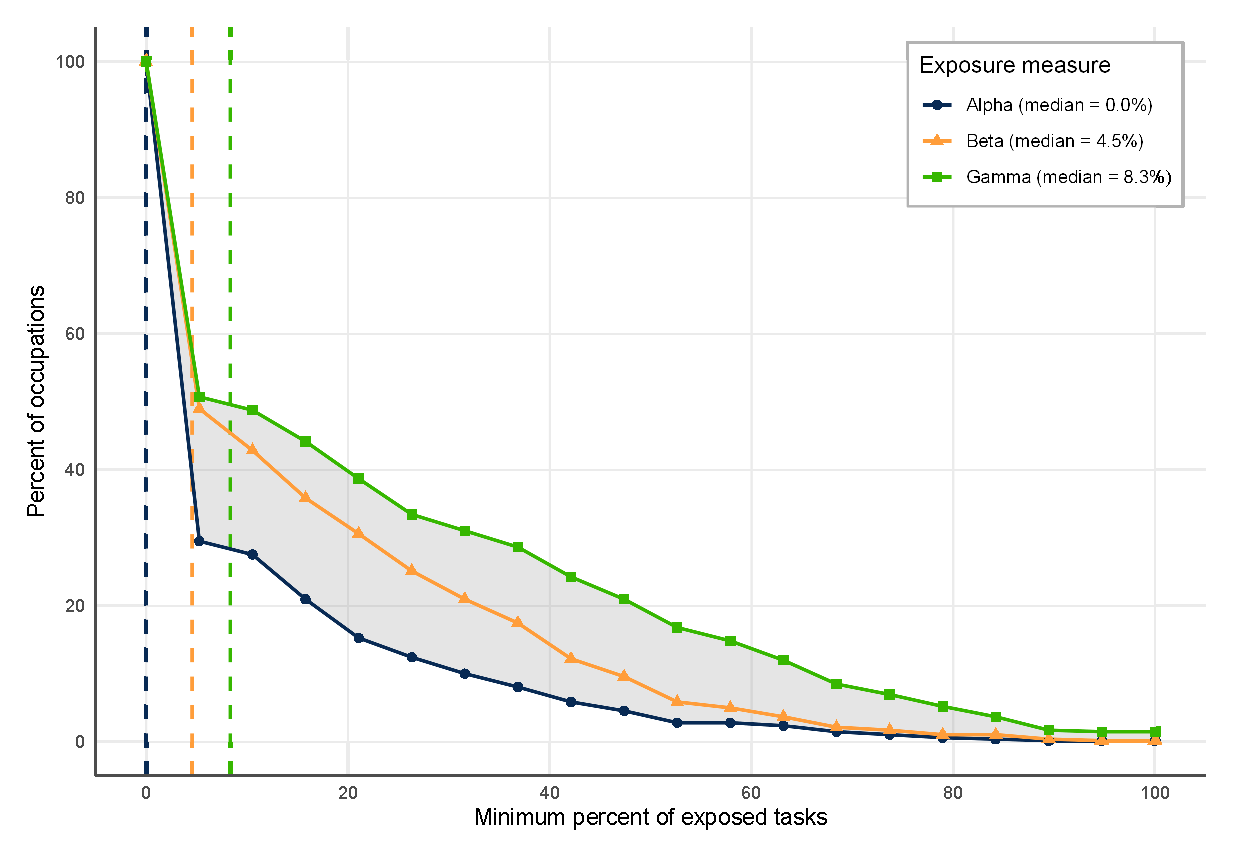
\includegraphics[width=\textwidth]{Figures/exposure_dist_gpt.eps}
    \caption{GPT-4o}
    \label{fig:exposure_dist_gpt}
  \end{subfigure}
  \medskip
  \begin{subfigure}[b]{0.7\textwidth}
    \centering
    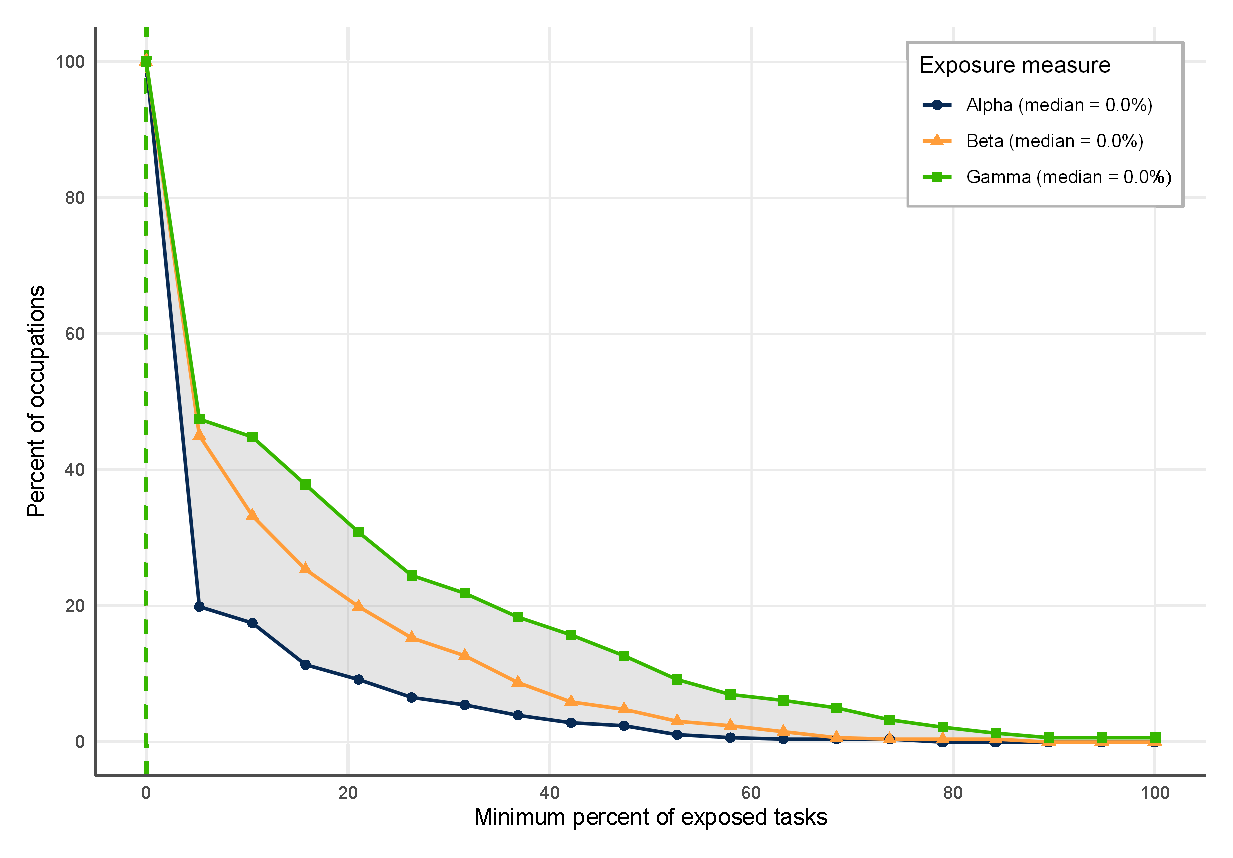
\includegraphics[width=\textwidth]{Figures/exposure_dist_human.eps}
    \caption{Human}
    \label{fig:exposure_dist_human}
  \end{subfigure}
  \medskip
  \label{fig:exposure_dist}
  \begin{minipage}{\textwidth}
    \small
    \textit{Note:} The plotted dashed lines indicate the median associated with each measure.
  \end{minipage}
\end{figure}


\begin{figure}[H]
  \centering
  \caption{Treatment group by exposure measure}
  \begin{subfigure}[b]{0.7\textwidth}
    \centering
    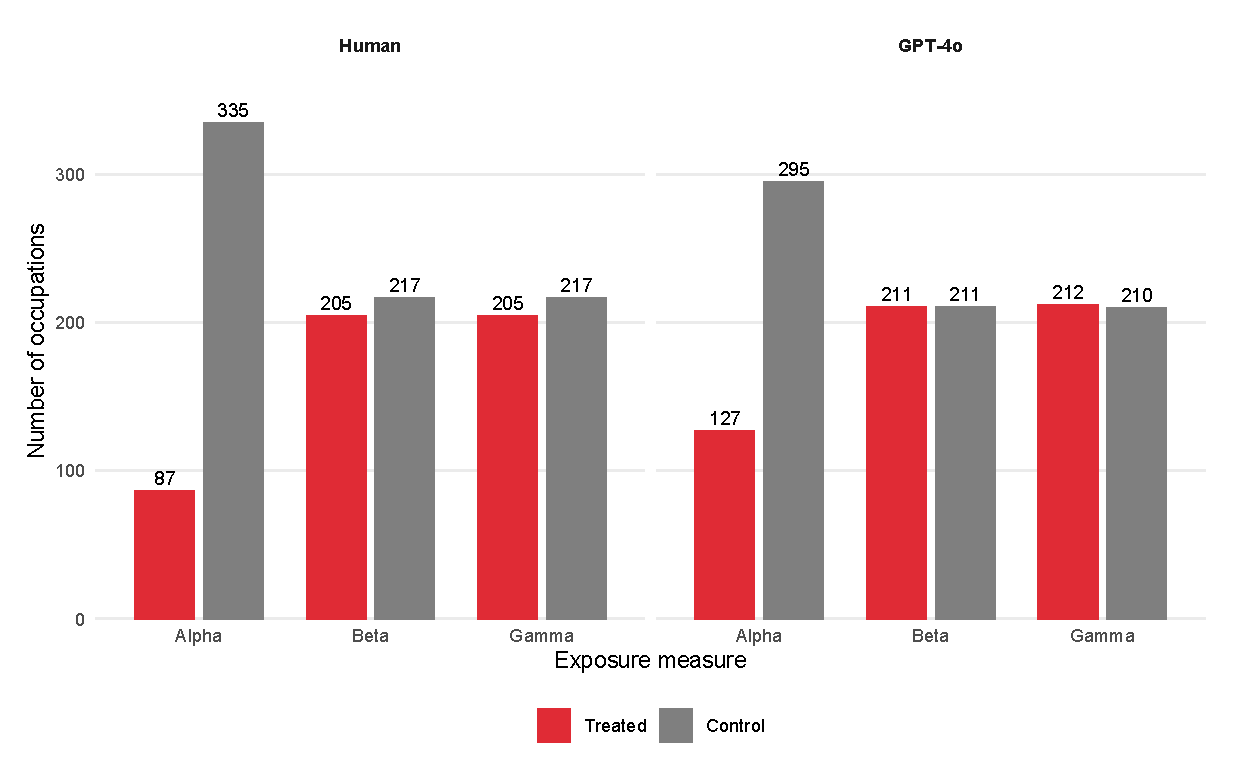
\includegraphics[width=\textwidth]{Figures/occupations_by_treatment.eps}
    \caption{Occupation}
    \label{fig:occupation_by_treat}
  \end{subfigure}
  \medskip
  \begin{subfigure}[b]{0.7\textwidth}
    \centering
    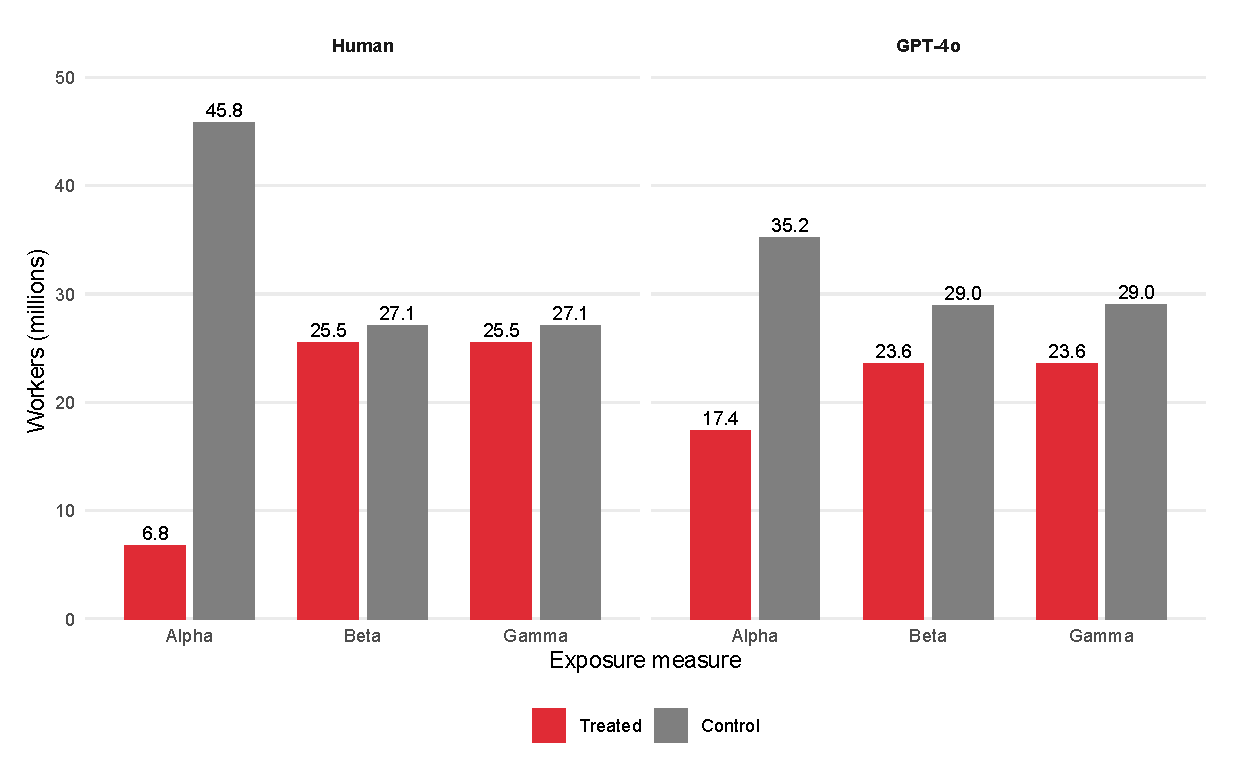
\includegraphics[width=\textwidth]{Figures/workers_by_treatment.eps}
    \caption{Workers}
    \label{fig:workers_by_treat}
  \end{subfigure}
  \medskip
  \label{fig:occupations_and_workers_by_treat}
  \begin{minipage}{\textwidth}
    \small
    \textit{Note:} Treated occupations are the ones above the median exposure. Number of workers are computed using the standard \glsxtrshort{ENOE} weights for the treatment quarter (2022 Q4).
  \end{minipage}
\end{figure}


\begin{figure}[H]
  \centering
  \caption{Overlap between treatment groups matrix}
  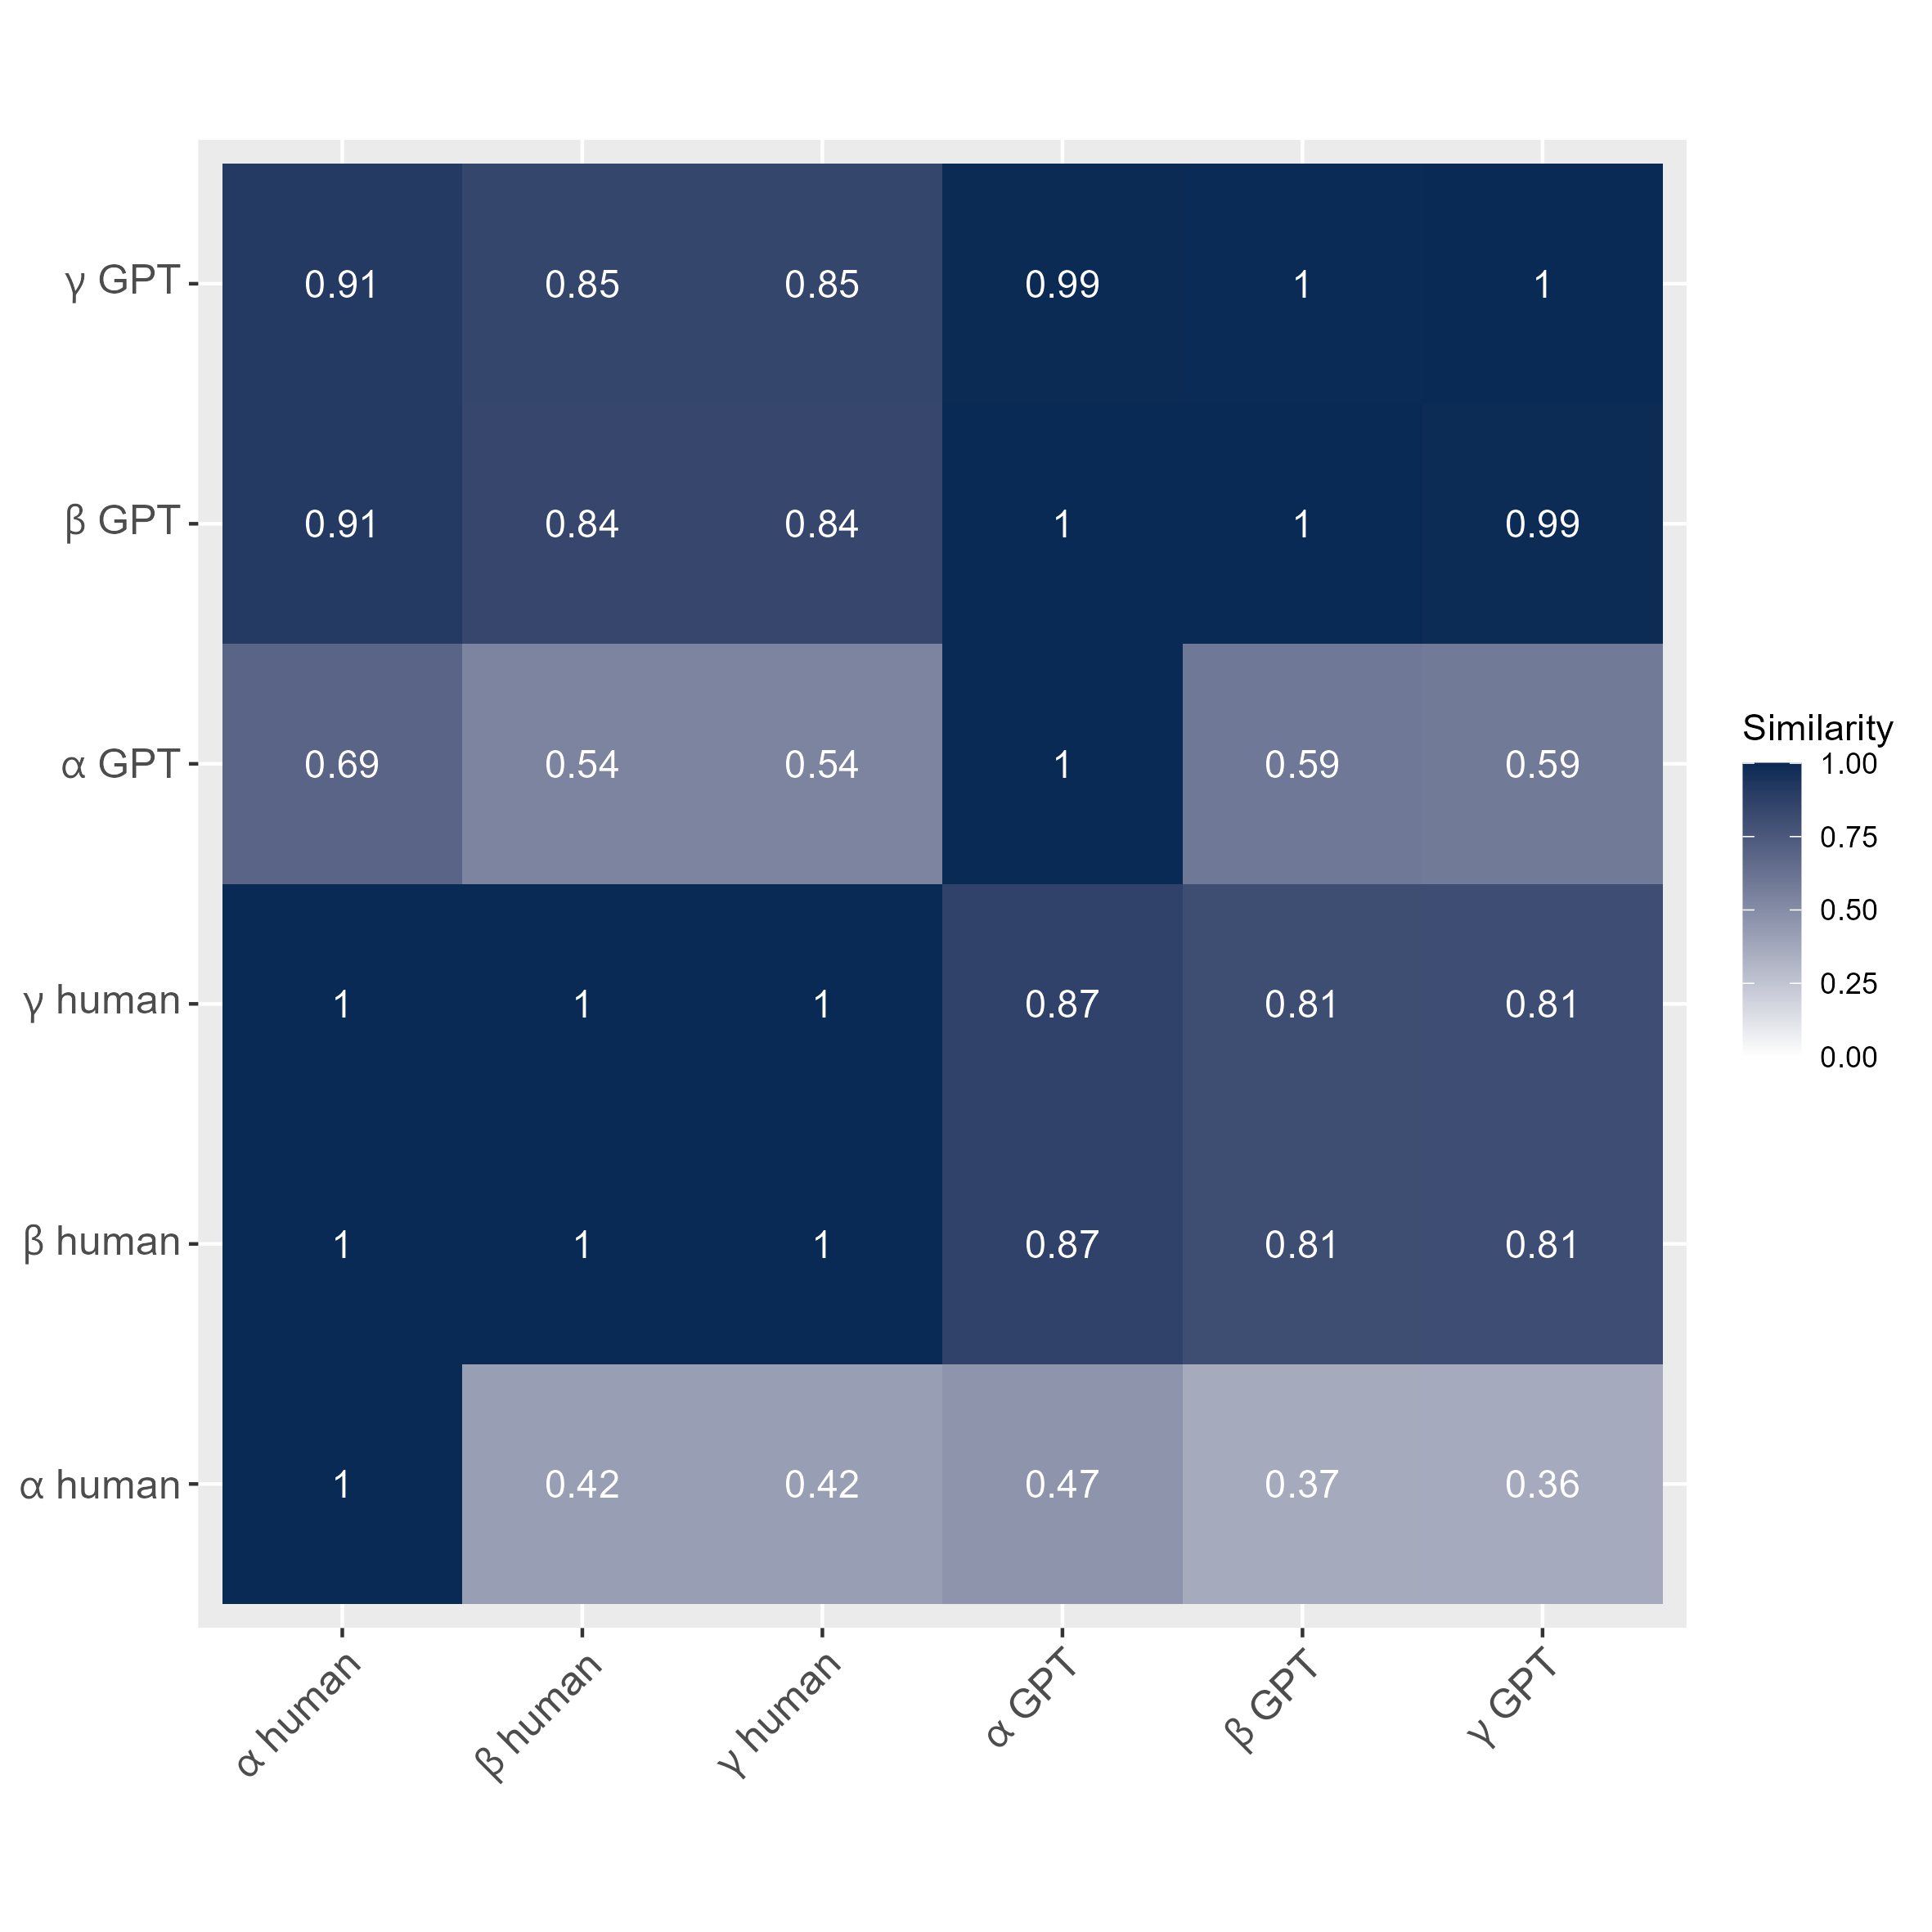
\includegraphics[width=0.7\linewidth]{Figures/matrix.png}
  \label{fig:matrix_overlap}
  \begin{minipage}{\textwidth}
    \small
    \textit{Note:} Share of occupations treated under the x axis measure that are also treated under the y axis measure.
  \end{minipage}
\end{figure}

\begin{table}[H]
  \centering
  \caption{\label{tab:imp_share_gpt}Share of imputed wages (\%) by quarter and treatment group (GPT-4o exposure)}
  \centering
  \resizebox{\ifdim\width>\linewidth\linewidth\else\width\fi}{!}{
    \begin{threeparttable}
      \begin{tabular}[t]{lcccc}
        \toprule
        \multicolumn{1}{c}{ } & \multicolumn{2}{c}{Alpha} & \multicolumn{2}{c}{Beta}                     \\
        \cmidrule(l{3pt}r{3pt}){2-3} \cmidrule(l{3pt}r{3pt}){4-5}
        Quarter               & Treated                   & Control                  & Treated & Control \\
        \midrule
        2020 Q3               & 37.5                      & 24.6                     & 36.7    & 22.4    \\
        2020 Q4               & 36.4                      & 23.6                     & 35.7    & 21.2    \\
        2021 Q1               & 34.7                      & 23.0                     & 34.2    & 20.7    \\
        2021 Q2               & 37.5                      & 25.0                     & 37.1    & 22.4    \\
        2021 Q3               & 37.8                      & 25.1                     & 37.5    & 22.5    \\
        \addlinespace
        2021 Q4               & 38.3                      & 25.5                     & 38.1    & 22.7    \\
        2022 Q1               & 36.0                      & 23.8                     & 35.5    & 21.4    \\
        2022 Q2               & 38.6                      & 25.3                     & 37.6    & 23.1    \\
        2022 Q3               & 39.4                      & 25.9                     & 38.7    & 23.4    \\
        2022 Q4               & 39.9                      & 25.8                     & 39.0    & 23.3    \\
        \addlinespace
        2023 Q1               & 39.0                      & 26.1                     & 38.5    & 23.6    \\
        2023 Q2               & 40.3                      & 26.4                     & 39.6    & 23.8    \\
        2023 Q3               & 39.8                      & 27.0                     & 39.4    & 24.4    \\
        2023 Q4               & 40.3                      & 27.4                     & 40.1    & 24.7    \\
        2024 Q1               & 38.7                      & 26.7                     & 38.3    & 24.2    \\
        \addlinespace
        2024 Q2               & 40.6                      & 27.8                     & 40.1    & 25.1    \\
        2024 Q3               & 40.9                      & 27.8                     & 40.3    & 25.4    \\
        2024 Q4               & 44.5                      & 30.6                     & 43.8    & 28.0    \\
        2025 Q1               & 47.3                      & 33.3                     & 47.0    & 30.4    \\
        2025 Q2               & 48.9                      & 35.3                     & 48.3    & 32.6    \\
        \addlinespace
        2025 Q3               & 48.9                      & 35.7                     & 48.6    & 32.9    \\
        2025 Q4               & 44.4                      & 31.8                     & 44.0    & 29.3    \\
        2026 Q1               & 37.2                      & 25.4                     & 36.8    & 23.0    \\
        2026 Q2               & 39.9                      & 27.3                     & 39.3    & 25.1    \\
        \bottomrule
      \end{tabular}
      \begin{tablenotes}
        \item \textit{Note: }  Share of workers whose earnings were imputed (PMM), weighted by survey expansion factors.
      \end{tablenotes}
    \end{threeparttable}}
\end{table}

\begin{table}[H]
  \centering
  \caption{\label{tab:imp_share_human} Share of imputed wages (\%) by quarter and treatment group (Human exposure)}
  \centering
  \resizebox{\ifdim\width>\linewidth\linewidth\else\width\fi}{!}{
    \begin{threeparttable}
      \begin{tabular}[t]{lcccc}
        \toprule
        \multicolumn{1}{c}{ } & \multicolumn{2}{c}{Alpha} & \multicolumn{2}{c}{Beta}                     \\
        \cmidrule(l{3pt}r{3pt}){2-3} \cmidrule(l{3pt}r{3pt}){4-5}
        Quarter               & Treated                   & Control                  & Treated & Control \\
        \midrule
        2020 Q3               & 43.1                      & 26.9                     & 35.4    & 23.0    \\
        2020 Q4               & 42.0                      & 25.8                     & 34.7    & 21.7    \\
        2021 Q1               & 40.0                      & 24.9                     & 33.2    & 21.1    \\
        2021 Q2               & 42.4                      & 27.2                     & 36.0    & 22.8    \\
        2021 Q3               & 43.3                      & 27.3                     & 36.1    & 23.1    \\
        \addlinespace
        2021 Q4               & 44.1                      & 27.5                     & 36.5    & 23.5    \\
        2022 Q1               & 41.9                      & 25.7                     & 33.9    & 22.3    \\
        2022 Q2               & 43.8                      & 27.6                     & 35.9    & 24.0    \\
        2022 Q3               & 45.9                      & 28.1                     & 37.1    & 24.0    \\
        2022 Q4               & 45.7                      & 28.1                     & 37.3    & 24.1    \\
        \addlinespace
        2023 Q1               & 44.7                      & 28.2                     & 36.8    & 24.4    \\
        2023 Q2               & 45.3                      & 28.9                     & 38.1    & 24.4    \\
        2023 Q3               & 45.3                      & 29.1                     & 38.2    & 24.7    \\
        2023 Q4               & 45.6                      & 29.6                     & 38.9    & 25.1    \\
        2024 Q1               & 43.9                      & 28.7                     & 36.7    & 25.0    \\
        \addlinespace
        2024 Q2               & 46.1                      & 29.9                     & 38.5    & 25.9    \\
        2024 Q3               & 47.2                      & 30.0                     & 38.9    & 25.9    \\
        2024 Q4               & 50.0                      & 33.1                     & 42.0    & 29.1    \\
        2025 Q1               & 52.2                      & 36.0                     & 44.9    & 31.8    \\
        2025 Q2               & 54.6                      & 37.7                     & 46.8    & 33.5    \\
        \addlinespace
        2025 Q3               & 54.1                      & 38.1                     & 47.1    & 33.7    \\
        2025 Q4               & 49.3                      & 34.1                     & 42.8    & 29.8    \\
        2026 Q1               & 42.9                      & 27.4                     & 35.6    & 23.6    \\
        2026 Q2               & 45.3                      & 29.6                     & 38.0    & 25.7    \\
        \bottomrule
      \end{tabular}
      \begin{tablenotes}
        \item \textit{Note: }Share of workers whose earnings were imputed (PMM), weighted by survey expansion factors.
      \end{tablenotes}
    \end{threeparttable}}
\end{table}

\begin{figure}[H]
  \centering
  \caption{Difference in imputed wage share}
  \begin{subfigure}[b]{0.7\textwidth}
    \centering
    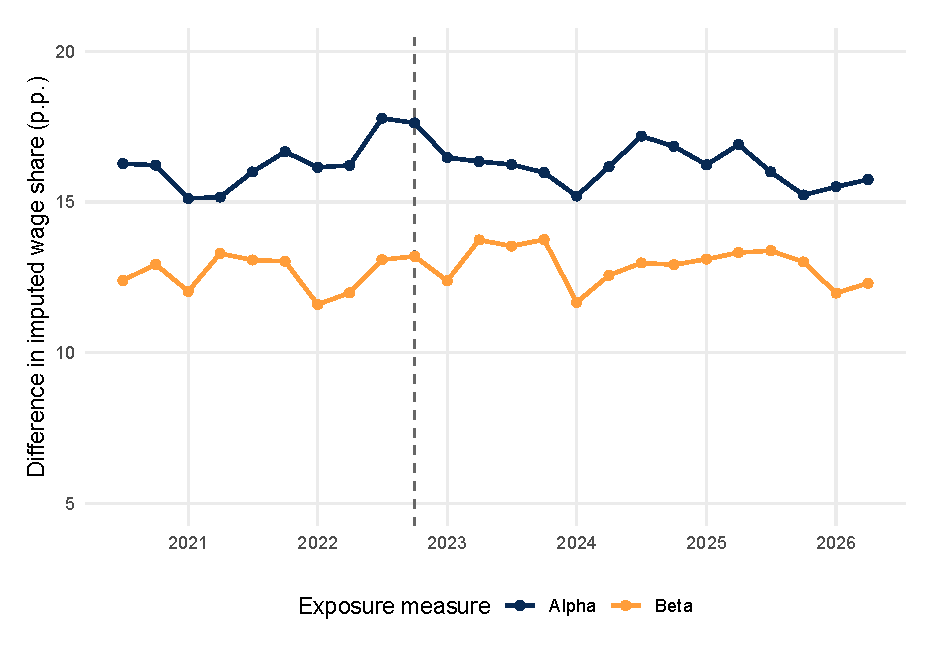
\includegraphics[width=\textwidth]{Figures/imp_share_gap_human.eps}
    \caption{Human}
    \label{fig:imp_share_gap_human}
  \end{subfigure}
  \medskip
  \begin{subfigure}[b]{0.7\textwidth}
    \centering
    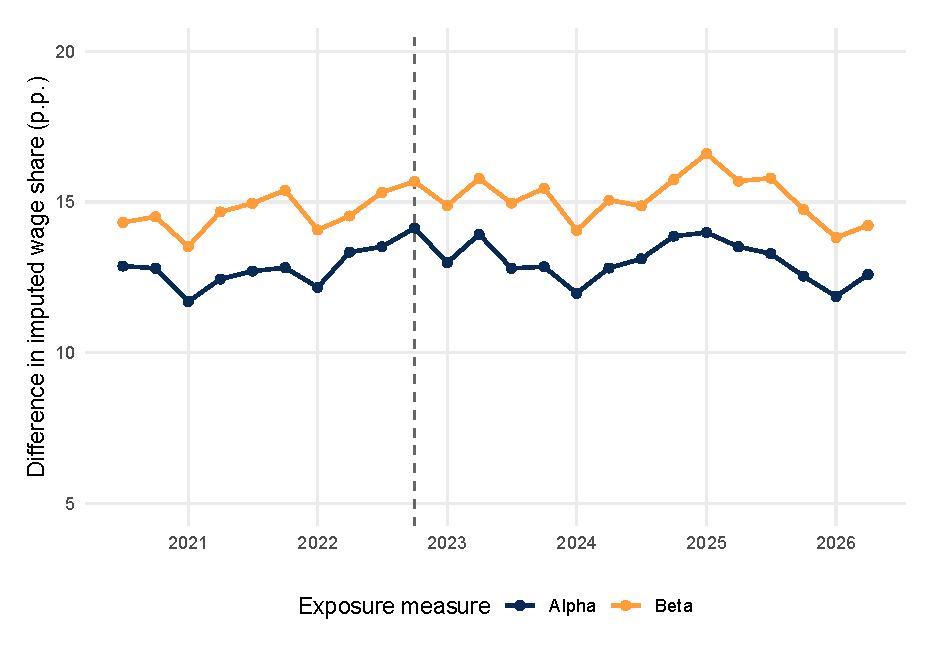
\includegraphics[width=\textwidth]{Figures/imp_share_gap_gpt.eps}
    \caption{GPT}
    \label{fig:imp_share_gap_gpt}
  \end{subfigure}
  \medskip
  \label{fig:imp_share_gap}
  \begin{minipage}{\textwidth}
    \small
    \textit{Note:} The figure plots the difference between treated and control occupations in the share of workers whose earnings were imputed (PMM). Panel (a) uses the human exposure measures and panel (b) the GPT-4o measures. Treated occupations are those above the median exposure. Shares are weighted by ENOE expansion factors. The dashed vertical line marks 2022 Q4, the quarter of ChatGPT's release. A flat series indicates that the gap in imputation between treated and control occupations remained constant before and after the treatment period.
  \end{minipage}
\end{figure}


\begin{table}[H]
  \centering
  \caption{\label{tab:sumstats_exposure_alpha_human}Summary statistics by treatment group (Human Alpha)}
  \centering
  \begin{threeparttable}
    \begin{tabular}[t]{lcccc}
      \toprule
      \multicolumn{1}{c}{ }          & \multicolumn{2}{c}{Control} & \multicolumn{2}{c}{Treated}                         \\
      \cmidrule(l{3pt}r{3pt}){2-3} \cmidrule(l{3pt}r{3pt}){4-5}
                                     & Before                      & After                       & Before    & After     \\
      \midrule
      Female (share)                 & 0.387                       & 0.404                       & 0.476     & 0.484     \\
                                     & (0.307)                     & (0.306)                     & (0.213)   & (0.214)   \\
      \addlinespace[3pt]
      Number of workers              & 910,742                     & 955,220                     & 266,830   & 276,887   \\
                                     & (881,588)                   & (949,268)                   & (194,607) & (203,653) \\
      \addlinespace[3pt]
      Number of informal workers     & 641,232                     & 654,980                     & 37,535    & 40,185    \\
                                     & (704,332)                   & (725,615)                   & (26,768)  & (26,522)  \\
      \addlinespace[3pt]
      Social security access (share) & 0.367                       & 0.373                       & 0.731     & 0.727     \\
                                     & (0.339)                     & (0.336)                     & (0.208)   & (0.206)   \\
      \addlinespace[3pt]
      Union member (share)           & 0.382                       & 0.361                       & 0.764     & 0.711     \\
                                     & (0.341)                     & (0.337)                     & (0.288)   & (0.325)   \\
      \addlinespace[3pt]
      Years of schooling             & 10.13                       & 10.42                       & 15.40     & 15.54     \\
                                     & (2.36)                      & (2.31)                      & (1.91)    & (1.97)    \\
      \addlinespace[3pt]
      Age (years)                    & 39.0                        & 39.4                        & 38.6      & 38.8      \\
                                     & (4.1)                       & (4.1)                       & (3.1)     & (3.0)     \\
      \addlinespace[3pt]
      Monthly earnings (MXN)         & 7,179                       & 9,546                       & 11,486    & 14,928    \\
                                     & (3,159)                     & (3,959)                     & (2,769)   & (3,662)   \\
      \addlinespace[3pt]
      Weekly hours worked            & 42.2                        & 41.9                        & 36.7      & 36.9      \\
                                     & (7.2)                       & (7.0)                       & (7.9)     & (7.5)     \\
      \midrule
      Occupations                    & 335                         & 335                         & 87        & 87        \\
      Occupation X quarters          & 3,350                       & 4,690                       & 870       & 1,218     \\
      \bottomrule
    \end{tabular}
    \begin{tablenotes}
      \item \textit{Note: } Occupation by quarter observations. Means weighted by occupation employment, with standard deviations across occupation quarters in parentheses. Treated occupations are the ones above the median exposure. The \textit{Before} column averages 2022 Q4 and earlier and the \textit{After} column 2023 Q1 onward. Monthly earnings are imputed with predictive mean matching (PMM).
    \end{tablenotes}
  \end{threeparttable}
\end{table}


\begin{table}[H]
  \centering
  \caption{\label{tab:sumstats_exposure_beta_human}Summary statistics by treatment group (Human Beta)}
  \centering
  \begin{threeparttable}
    \begin{tabular}[t]{lcccc}
      \toprule
      \multicolumn{1}{c}{ }          & \multicolumn{2}{c}{Control} & \multicolumn{2}{c}{Treated}                             \\
      \cmidrule(l{3pt}r{3pt}){2-3} \cmidrule(l{3pt}r{3pt}){4-5}
                                     & Before                      & After                       & Before      & After       \\
      \midrule
      Female (share)                 & 0.326                       & 0.342                       & 0.476       & 0.491       \\
                                     & (0.323)                     & (0.327)                     & (0.245)     & (0.238)     \\
      \addlinespace[3pt]
      Number of workers              & 727,482                     & 740,650                     & 938,749     & 1,005,057   \\
                                     & (628,573)                   & (614,919)                   & (1,032,570) & (1,140,656) \\
      \addlinespace[3pt]
      Number of informal workers     & 559,929                     & 552,992                     & 570,065     & 601,717     \\
                                     & (631,402)                   & (606,973)                   & (744,545)   & (801,228)   \\
      \addlinespace[3pt]
      Social security access (share) & 0.351                       & 0.355                       & 0.480       & 0.486       \\
                                     & (0.337)                     & (0.335)                     & (0.345)     & (0.338)     \\
      \addlinespace[3pt]
      Union member (share)           & 0.344                       & 0.327                       & 0.540       & 0.504       \\
                                     & (0.335)                     & (0.329)                     & (0.357)     & (0.363)     \\
      \addlinespace[3pt]
      Years of schooling             & 9.49                        & 9.78                        & 12.20       & 12.46       \\
                                     & (2.03)                      & (1.96)                      & (3.04)      & (2.97)      \\
      \addlinespace[3pt]
      Age (years)                    & 39.1                        & 39.7                        & 38.7        & 39.0        \\
                                     & (3.8)                       & (3.8)                       & (4.1)       & (4.2)       \\
      \addlinespace[3pt]
      Monthly earnings (MXN)         & 6,964                       & 9,304                       & 8,542       & 11,220      \\
                                     & (2,874)                     & (3,625)                     & (3,767)     & (4,747)     \\
      \addlinespace[3pt]
      Weekly hours worked            & 42.0                        & 41.8                        & 40.9        & 40.7        \\
                                     & (7.9)                       & (7.9)                       & (7.1)       & (6.5)       \\
      \midrule
      Occupations                    & 217                         & 217                         & 205         & 205         \\
      Occupation X quarters          & 2,170                       & 3,038                       & 2,050       & 2,870       \\
      \bottomrule
    \end{tabular}
    \begin{tablenotes}
      \item \textit{Note: } Occupation by quarter observations. Means weighted by occupation employment, with standard deviations across occupation quarters in parentheses. Treated occupations are the ones above the median exposure. The \textit{Before} column averages 2022 Q4 and earlier and the \textit{After} column 2023 Q1 onward. Monthly earnings are imputed with predictive mean matching (PMM).
    \end{tablenotes}
  \end{threeparttable}
\end{table}


\begin{table}[H]
  \centering
  \caption{\label{tab:sumstats_exposure_alpha_gpt}Summary statistics by treatment group (GPT-4o Alpha)}
  \centering
  \begin{threeparttable}
    \begin{tabular}[t]{lcccc}
      \toprule
      \multicolumn{1}{c}{ }          & \multicolumn{2}{c}{Control} & \multicolumn{2}{c}{Treated}                             \\
      \cmidrule(l{3pt}r{3pt}){2-3} \cmidrule(l{3pt}r{3pt}){4-5}
                                     & Before                      & After                       & Before      & After       \\
      \midrule
      Female (share)                 & 0.353                       & 0.372                       & 0.491       & 0.497       \\
                                     & (0.308)                     & (0.310)                     & (0.252)     & (0.249)     \\
      \addlinespace[3pt]
      Number of workers              & 811,660                     & 814,892                     & 865,035     & 976,131     \\
                                     & (763,183)                   & (762,852)                   & (1,013,469) & (1,159,948) \\
      \addlinespace[3pt]
      Number of informal workers     & 637,376                     & 629,072                     & 416,923     & 471,927     \\
                                     & (677,286)                   & (668,627)                   & (686,690)   & (770,522)   \\
      \addlinespace[3pt]
      Social security access (share) & 0.294                       & 0.299                       & 0.655       & 0.656       \\
                                     & (0.328)                     & (0.326)                     & (0.246)     & (0.237)     \\
      \addlinespace[3pt]
      Union member (share)           & 0.324                       & 0.309                       & 0.639       & 0.591       \\
                                     & (0.332)                     & (0.325)                     & (0.315)     & (0.338)     \\
      \addlinespace[3pt]
      Years of schooling             & 9.60                        & 9.91                        & 13.23       & 13.40       \\
                                     & (2.29)                      & (2.27)                      & (2.45)      & (2.39)      \\
      \addlinespace[3pt]
      Age (years)                    & 39.6                        & 40.0                        & 37.7        & 38.0        \\
                                     & (4.1)                       & (4.1)                       & (3.4)       & (3.3)       \\
      \addlinespace[3pt]
      Monthly earnings (MXN)         & 6,886                       & 9,168                       & 9,432       & 12,356      \\
                                     & (3,051)                     & (3,875)                     & (3,513)     & (4,360)     \\
      \addlinespace[3pt]
      Weekly hours worked            & 41.9                        & 41.4                        & 40.7        & 41.0        \\
                                     & (7.4)                       & (7.3)                       & (7.9)       & (7.3)       \\
      \midrule
      Occupations                    & 295                         & 295                         & 127         & 127         \\
      Occupation X quarters          & 2,950                       & 4,130                       & 1,270       & 1,778       \\
      \bottomrule
    \end{tabular}
    \begin{tablenotes}
      \item \textit{Note: } Occupation by quarter observations. Means weighted by occupation employment, with standard deviations across occupation quarters in parentheses. Treated occupations are the ones above the median exposure. The \textit{Before} column averages 2022 Q4 and earlier and the \textit{After} column 2023 Q1 onward. Monthly earnings are imputed with predictive mean matching (PMM).
    \end{tablenotes}
  \end{threeparttable}
\end{table}

\begin{table}[H]
  \centering
  \caption{\label{tab:sumstats_exposure_beta_gpt}Summary statistics by treatment group (GPT-4o Beta)}
  \centering
  \begin{threeparttable}
    \begin{tabular}[t]{lcccc}
      \toprule
      \multicolumn{1}{c}{ }          & \multicolumn{2}{c}{Control} & \multicolumn{2}{c}{Treated}                             \\
      \cmidrule(l{3pt}r{3pt}){2-3} \cmidrule(l{3pt}r{3pt}){4-5}
                                     & Before                      & After                       & Before      & After       \\
      \midrule
      Female (share)                 & 0.350                       & 0.371                       & 0.459       & 0.466       \\
                                     & (0.321)                     & (0.323)                     & (0.254)     & (0.252)     \\
      \addlinespace[3pt]
      Number of workers              & 753,795                     & 749,141                     & 922,104     & 1,013,118   \\
                                     & (632,711)                   & (604,240)                   & (1,057,845) & (1,175,229) \\
      \addlinespace[3pt]
      Number of informal workers     & 612,756                     & 593,143                     & 505,779     & 556,618     \\
                                     & (636,482)                   & (602,674)                   & (742,810)   & (817,171)   \\
      \addlinespace[3pt]
      Social security access (share) & 0.294                       & 0.299                       & 0.559       & 0.563       \\
                                     & (0.326)                     & (0.323)                     & (0.315)     & (0.309)     \\
      \addlinespace[3pt]
      Union member (share)           & 0.296                       & 0.282                       & 0.623       & 0.578       \\
                                     & (0.318)                     & (0.310)                     & (0.323)     & (0.344)     \\
      \addlinespace[3pt]
      Years of schooling             & 9.20                        & 9.52                        & 12.75       & 12.96       \\
                                     & (1.96)                      & (1.95)                      & (2.66)      & (2.58)      \\
      \addlinespace[3pt]
      Age (years)                    & 39.1                        & 39.6                        & 38.7        & 39.0        \\
                                     & (4.1)                       & (4.2)                       & (3.8)       & (3.8)       \\
      \addlinespace[3pt]
      Monthly earnings (MXN)         & 6,273                       & 8,399                       & 9,511       & 12,446      \\
                                     & (2,111)                     & (2,699)                     & (3,863)     & (4,829)     \\
      \addlinespace[3pt]
      Weekly hours worked            & 41.2                        & 40.8                        & 41.8        & 41.8        \\
                                     & (7.7)                       & (7.6)                       & (7.4)       & (6.8)       \\
      \midrule
      Occupations                    & 211                         & 211                         & 211         & 211         \\
      Occupation X quarters          & 2,110                       & 2,954                       & 2,110       & 2,954       \\
      \bottomrule
    \end{tabular}
    \begin{tablenotes}
      \item \textit{Note: } Occupation by quarter observations. Means weighted by occupation employment, with standard deviations across occupation quarters in parentheses. Treated occupations are the ones above the median exposure. The \textit{Before} column averages 2022 Q4 and earlier and the \textit{After} column 2023 Q1 onward. Monthly earnings are imputed with predictive mean matching (PMM).
    \end{tablenotes}
  \end{threeparttable}
\end{table}


\begin{figure}[H]
  \centering
  \caption{Imputed monthly earnings density distribution across occupations by treatment group}
  \begin{subfigure}[b]{0.49\textwidth}
    \centering
    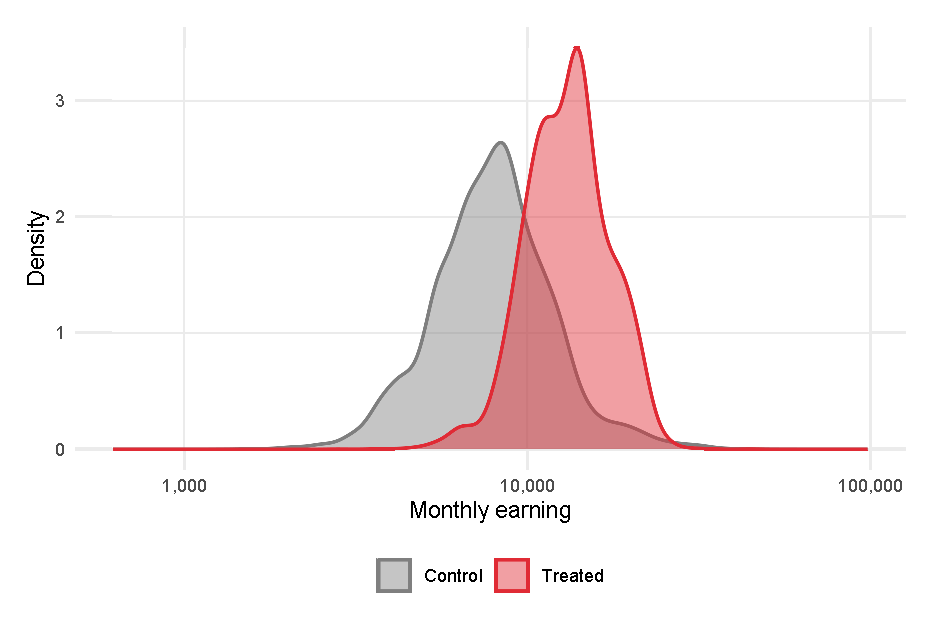
\includegraphics[width=\textwidth]{Figures/dist_wage_imp_alpha_human.eps}
    \caption{$\alpha$ human}
    \label{fig:dist_wage_imp_alpha_human}
  \end{subfigure}
  \hfill
  \begin{subfigure}[b]{0.49\textwidth}
    \centering
    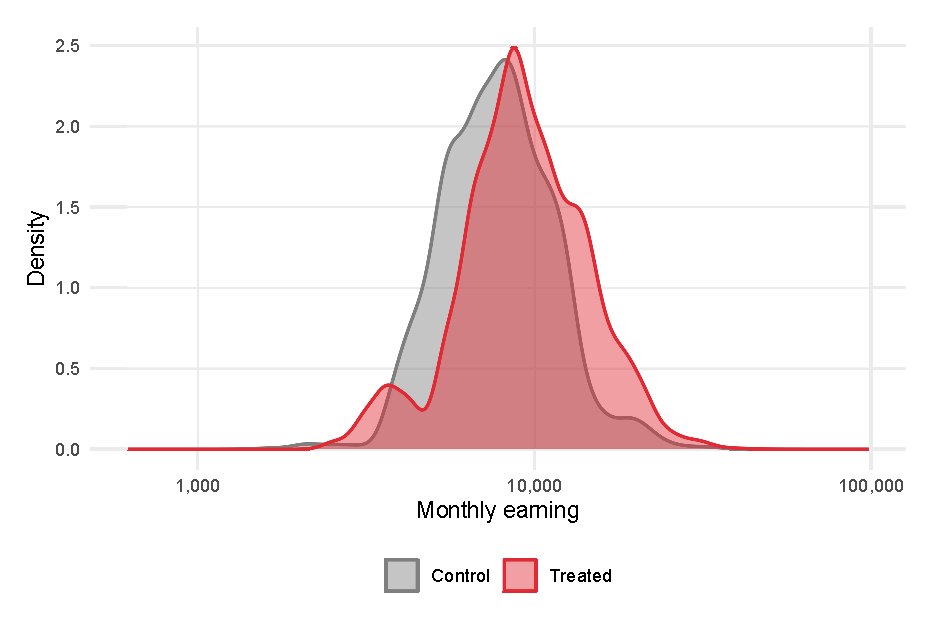
\includegraphics[width=\textwidth]{Figures/dist_wage_imp_beta_human.eps}
    \caption{$\beta$ human}
    \label{fig:dist_wage_imp_beta_human}
  \end{subfigure}
  \hfill
  \begin{subfigure}[b]{0.49\textwidth}
    \centering
    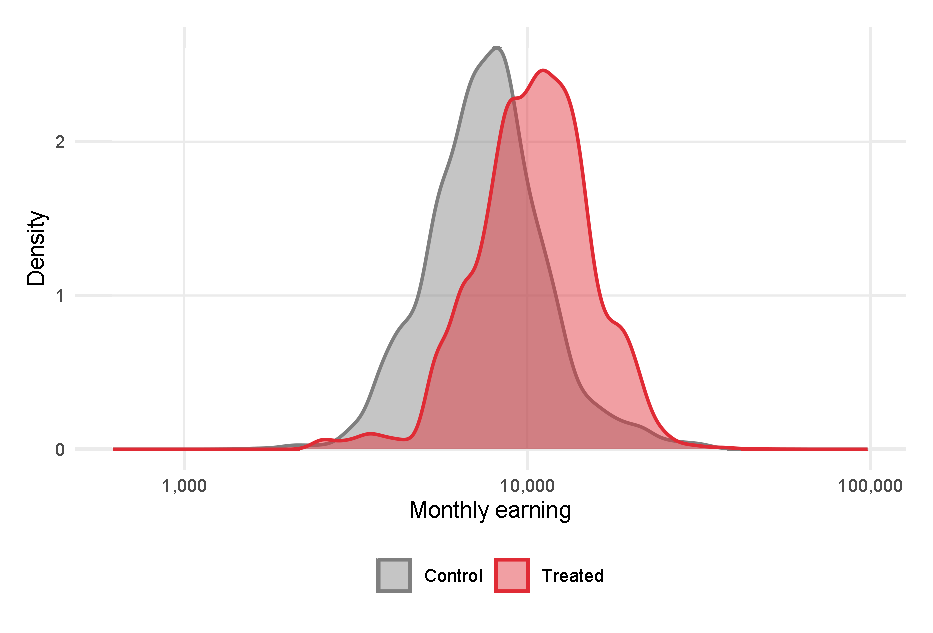
\includegraphics[width=\textwidth]{Figures/dist_wage_imp_alpha_gpt.eps}
    \caption{$\alpha$ GPT-4o}
    \label{fig:dist_wage_imp_alpha_gpt}
  \end{subfigure}
  \hfill
  \begin{subfigure}[b]{0.49\textwidth}
    \centering
    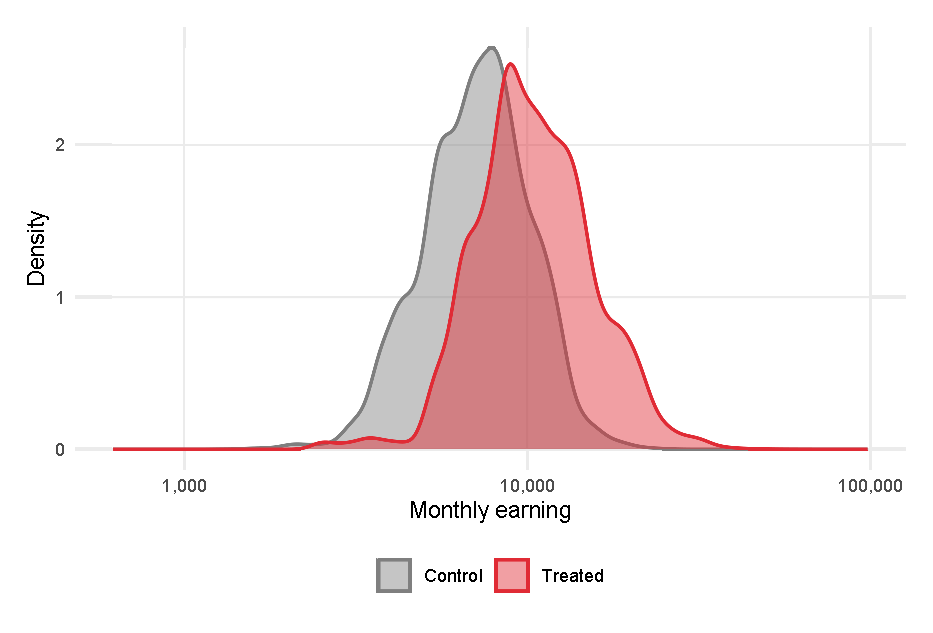
\includegraphics[width=\textwidth]{Figures/dist_wage_imp_beta_gpt.eps}
    \caption{$\beta$ GPT-4o}
    \label{fig:dist_wage_imp_beta_gpt}
  \end{subfigure}
  \hfill
  \label{fig:wage_dist}
  \begin{minipage}{0.6\textwidth}
    \small
    \textit{Note:} Kernel density of imputed monthly earnings (MXN, log scale), by treatment group, with weights by number of workers and averaged across the before and after treatment periods.
  \end{minipage}
\end{figure}

\begin{figure}[H]
  \centering
  \caption{Trends in monthly earnings by treatment group}
  \label{fig:trend_wage_imp}
  \begin{subfigure}[b]{0.49\textwidth}
    \centering
    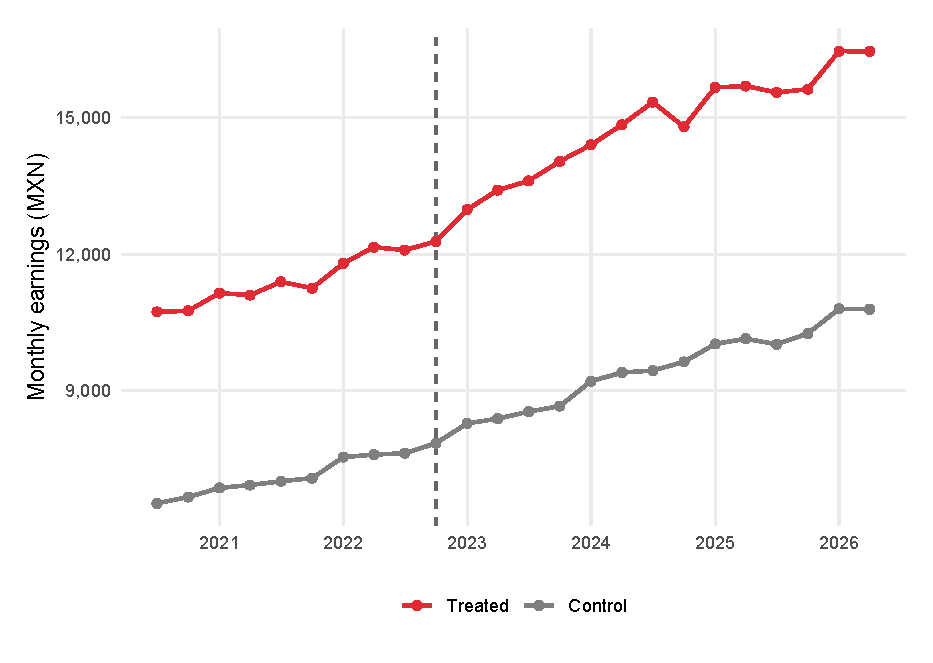
\includegraphics[width=\textwidth]{Figures/trend_wage_imp_alpha_human.eps}
    \caption{Human alpha}
    \label{fig:trend_wage_imp_human_alpha}
  \end{subfigure}
  \hfill
  \begin{subfigure}[b]{0.49\textwidth}
    \centering
    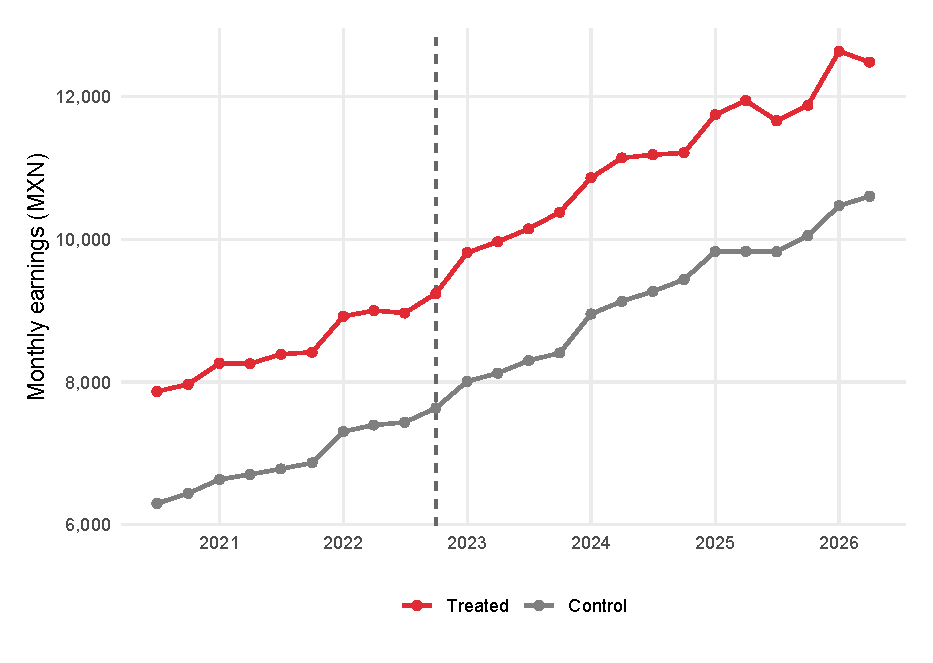
\includegraphics[width=\textwidth]{Figures/trend_wage_imp_beta_human.eps}
    \caption{Human beta}
    \label{fig:trend_wage_imp_beta_human}
  \end{subfigure}
  \hfill
  \begin{subfigure}[b]{0.49\textwidth}
    \centering
    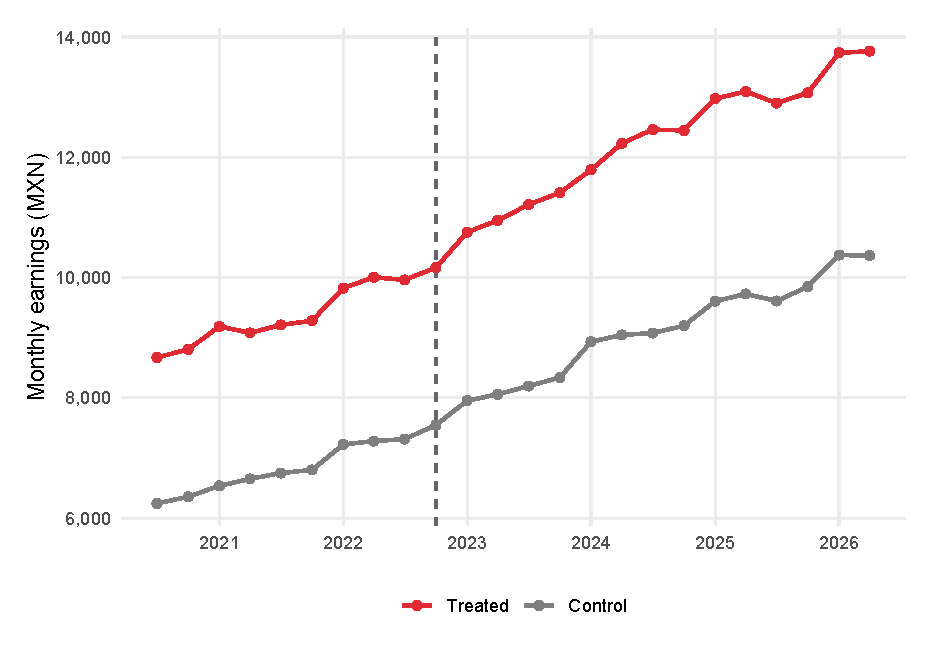
\includegraphics[width=\textwidth]{Figures/trend_wage_imp_alpha_gpt.eps}
    \caption{GPT-4o alpha}
    \label{fig:trend_wage_imp_gpt_alpha}
  \end{subfigure}
  \hfill
  \begin{subfigure}[b]{0.49\textwidth}
    \centering
    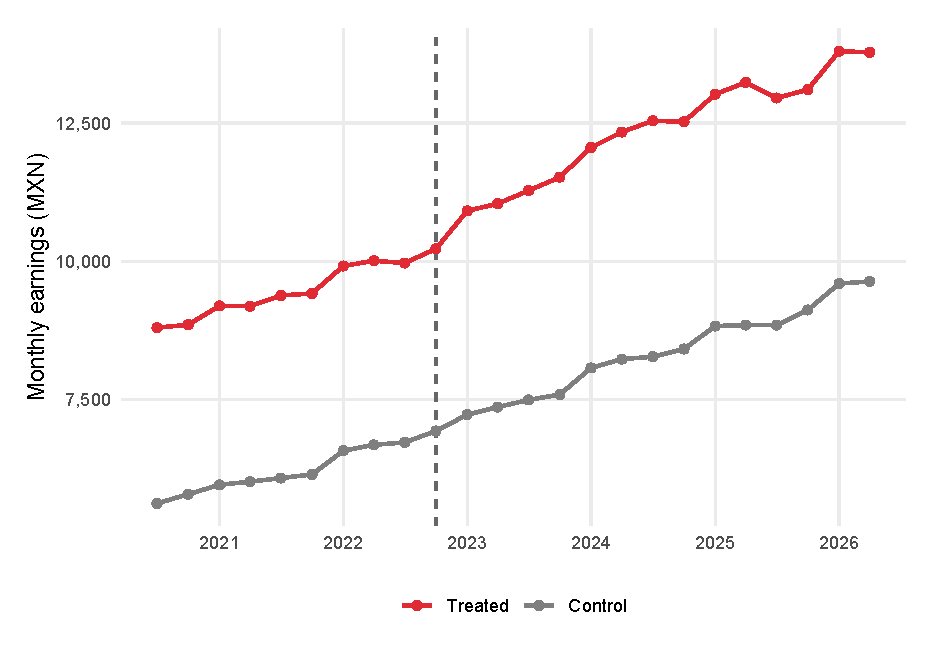
\includegraphics[width=\textwidth]{Figures/trend_wage_imp_beta_gpt.eps}
    \caption{GPT-4o beta}
    \label{fig:trend_wage_imp_gpt_beta}
  \end{subfigure}
  \hfill
  \begin{minipage}{\textwidth}
    \small
    \textit{Note:} The figure displays trends of monthly earnings in treated and control occupations over time. Panel (a) and (b) use the human exposure measure, while panel (c) and (d) use the GPT-4o exposure measure.
  \end{minipage}
\end{figure}

\begin{figure}[H]
  \centering
  \caption{Trends on the logarithm of the number of workers by treatment group}
  \label{fig:trend_workers_imp}
  \begin{subfigure}[b]{0.49\textwidth}
    \centering
    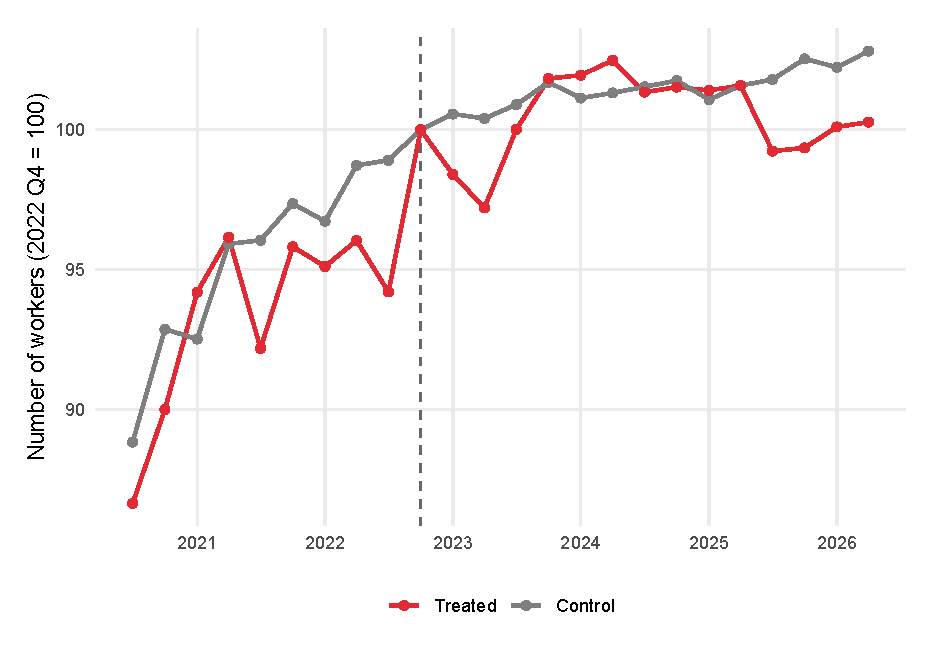
\includegraphics[width=\textwidth]{Figures/trend_n_pop_alpha_human.eps}
    \caption{Human alpha}
    \label{fig:trend_workers_imp_human_alpha}
  \end{subfigure}
  \hfill
  \begin{subfigure}[b]{0.49\textwidth}
    \centering
    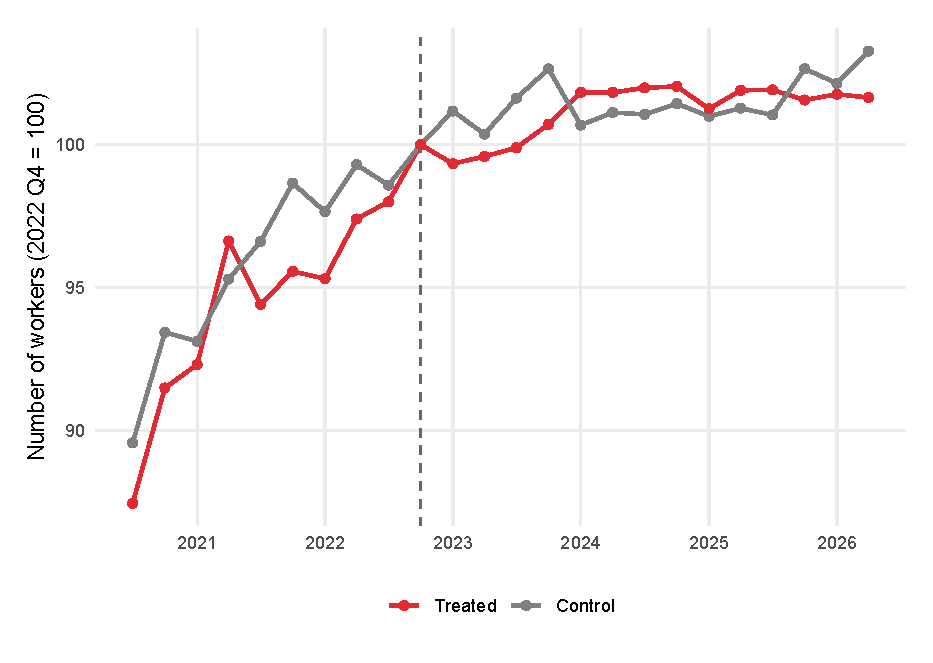
\includegraphics[width=\textwidth]{Figures/trend_n_pop_beta_human.eps}
    \caption{Human beta}
    \label{fig:trend_workers_imp_beta_human}
  \end{subfigure}
  \hfill
  \begin{subfigure}[b]{0.49\textwidth}
    \centering
    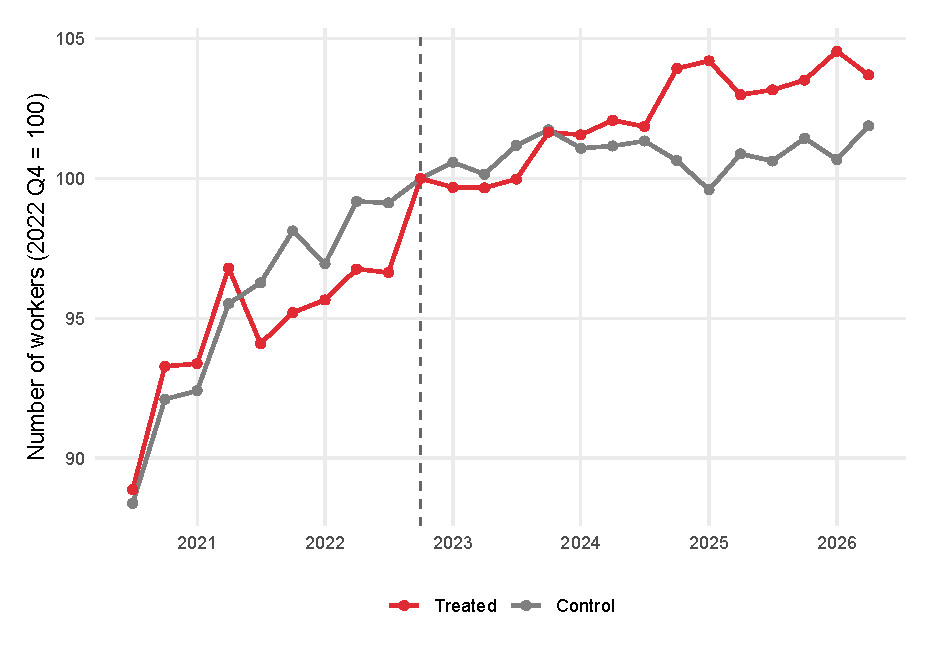
\includegraphics[width=\textwidth]{Figures/trend_n_pop_alpha_gpt.eps}
    \caption{GPT-4o alpha}
    \label{fig:trend_workers_imp_gpt_alpha}
  \end{subfigure}
  \hfill
  \begin{subfigure}[b]{0.49\textwidth}
    \centering
    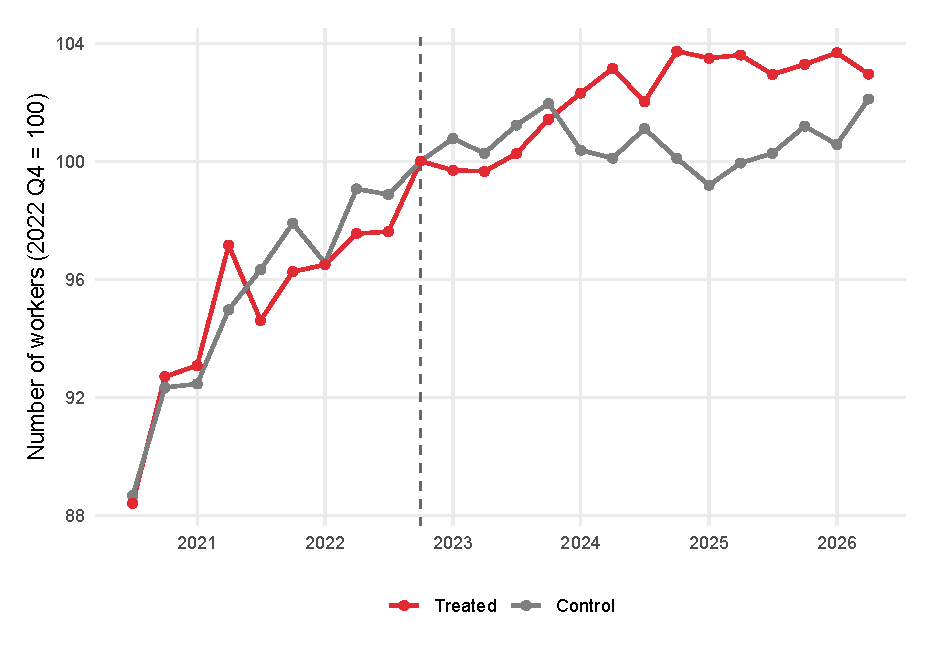
\includegraphics[width=\textwidth]{Figures/trend_n_pop_beta_gpt.eps}
    \caption{GPT-4o beta}
    \label{fig:trend_workers_imp_gpt_beta}
  \end{subfigure}
  \hfill
  \begin{minipage}{\textwidth}
    \small
    \textit{Note:} The figure displays trends for the number of workers in treated and control occupations over time. Panel (a) and (b) use the human exposure measure, while panel (c) and (d) use the GPT-4o exposure measure.
  \end{minipage}
\end{figure}

\begin{figure}[H]
  \centering
  \caption{Trends on the logarithm of the number of informal workers by treatment group}
  \label{fig:trend_informal_imp}
  \begin{subfigure}[b]{0.49\textwidth}
    \centering
    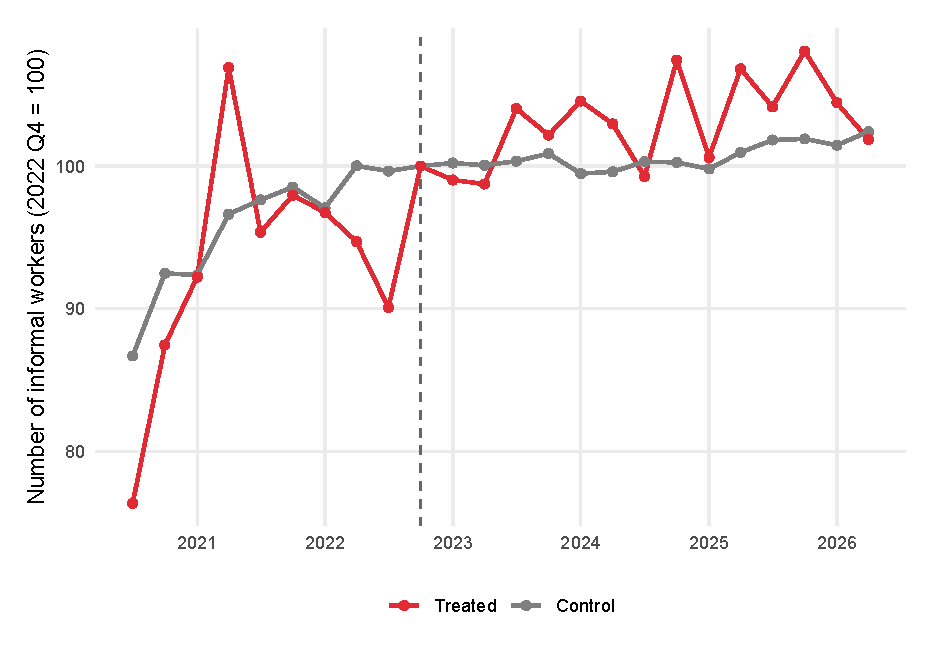
\includegraphics[width=\textwidth]{Figures/trend_informal_alpha_human.eps}
    \caption{Human alpha}
    \label{fig:trend_informal_imp_human_alpha}
  \end{subfigure}
  \hfill
  \begin{subfigure}[b]{0.49\textwidth}
    \centering
    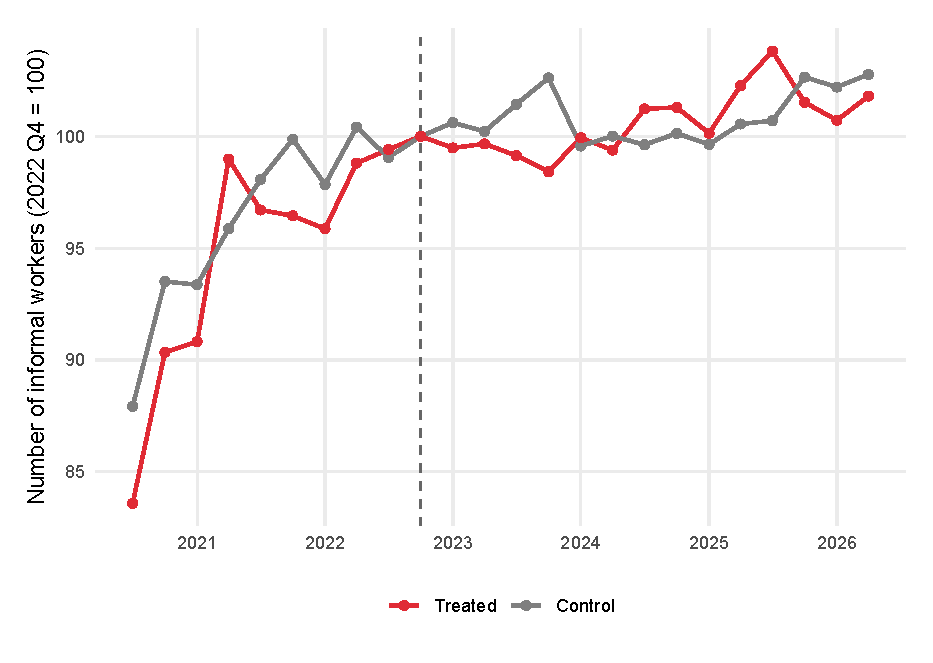
\includegraphics[width=\textwidth]{Figures/trend_informal_beta_human.eps}
    \caption{Human beta}
    \label{fig:trend_informal_imp_beta_human}
  \end{subfigure}
  \hfill
  \begin{subfigure}[b]{0.49\textwidth}
    \centering
    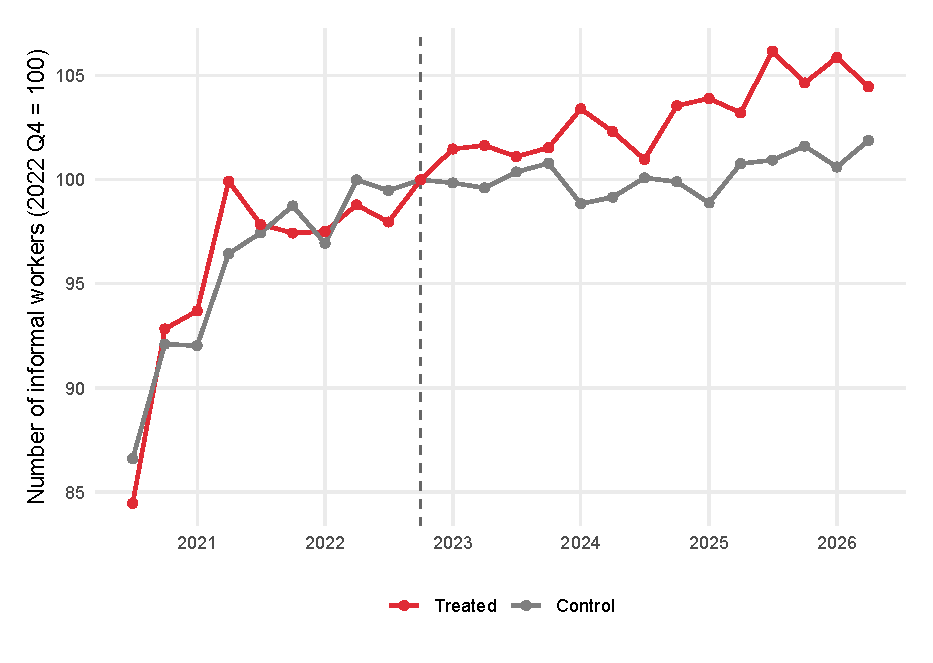
\includegraphics[width=\textwidth]{Figures/trend_informal_alpha_gpt.eps}
    \caption{GPT-4o alpha}
    \label{fig:trend_informal_imp_gpt_alpha}
  \end{subfigure}
  \hfill
  \begin{subfigure}[b]{0.49\textwidth}
    \centering
    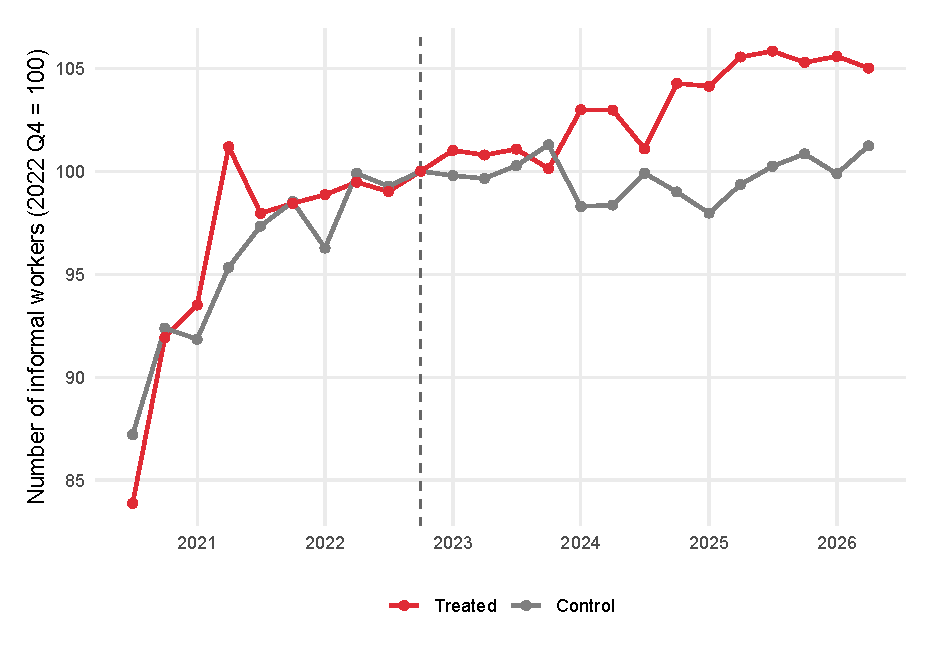
\includegraphics[width=\textwidth]{Figures/trend_informal_beta_gpt.eps}
    \caption{GPT-4o beta}
    \label{fig:trend_informal_imp_gpt_beta}
  \end{subfigure}
  \hfill
  \begin{minipage}{\textwidth}
    \small
    \textit{Note:} The figure displays trends for the number of informal workers in treated and control occupations over time. Panel (a) and (b) use the human exposure measure, while panel (c) and (d) use the GPT-4o exposure measure.
  \end{minipage}
\end{figure}




\begin{table}[H]
  \centering
  \caption{\label{tab:did_main}Difference in differences estimates: effect of ChatGPT's release on labor market outcomes}
  \centering
  \resizebox{\ifdim\width>\linewidth\linewidth\else\width\fi}{!}{
    \begin{threeparttable}
      \begin{tabular}[t]{lcccc}
        \toprule
                                       & Log number of workers & Log number of informal workers & Monthly earnings (MXN) & Share of imputed wages (\%) \\
        \midrule
        \addlinespace[0.3em]
        \multicolumn{5}{l}{\textbf{Panel A: Human exposure}}                                                                                           \\
        \addlinespace[0.3em]
        \multicolumn{5}{l}{\textit{Beta}}                                                                                                              \\
        \hspace{1em}Treated x Post     & 0.004                 & 0.042                          & 259.091                & 0.526                       \\
        \hspace{1em}                   & (0.023)               & (0.027)                        & (193.619)              & (0.346)                     \\
        \hspace{1em}Female (share)     & 0.107                 & 0.250**                        & -1103.525**            & -3.700**                    \\
        \hspace{1em}                   & (0.075)               & (0.118)                        & (533.885)              & (1.646)                     \\
        \hspace{1em}Years of schooling & 0.002                 & -0.024                         & 155.285***             & 0.808***                    \\
        \hspace{1em}                   & (0.008)               & (0.016)                        & (38.079)               & (0.157)                     \\
        \hspace{1em}Age (years)        & -0.011**              & -0.018***                      & 10.462                 & 0.190***                    \\
        \hspace{1em}                   & (0.006)               & (0.005)                        & (19.250)               & (0.067)                     \\
        \addlinespace[0.3em]
        \multicolumn{5}{l}{\textit{Alpha}}                                                                                                             \\
        \hspace{1em}Treated x Post     & -0.006                & 0.072*                         & 1011.201***            & -0.290                      \\
        \hspace{1em}                   & (0.040)               & (0.038)                        & (191.886)              & (0.415)                     \\
        \hspace{1em}Female (share)     & 0.109                 & 0.255**                        & -1116.064**            & -3.559**                    \\
        \hspace{1em}                   & (0.075)               & (0.119)                        & (500.374)              & (1.666)                     \\
        \hspace{1em}Years of schooling & 0.002                 & -0.023                         & 174.504***             & 0.786***                    \\
        \hspace{1em}                   & (0.007)               & (0.016)                        & (38.070)               & (0.155)                     \\
        \hspace{1em}Age (years)        & -0.011*               & -0.018***                      & 17.331                 & 0.184***                    \\
        \hspace{1em}                   & (0.006)               & (0.005)                        & (18.755)               & (0.067)                     \\
        \addlinespace[0.3em]
        \multicolumn{5}{l}{\textbf{Panel B: GPT-4o exposure}}                                                                                          \\
        \addlinespace[0.3em]
        \multicolumn{5}{l}{\textit{Alpha}}                                                                                                             \\
        \hspace{1em}Treated x Post     & 0.016                 & 0.056**                        & 625.079***             & 0.427                       \\
        \hspace{1em}                   & (0.024)               & (0.026)                        & (218.555)              & (0.344)                     \\
        \hspace{1em}Female (share)     & 0.105                 & 0.248**                        & -1182.879**            & -3.674**                    \\
        \hspace{1em}                   & (0.074)               & (0.117)                        & (523.082)              & (1.655)                     \\
        \hspace{1em}Years of schooling & 0.002                 & -0.023                         & 162.929***             & 0.804***                    \\
        \hspace{1em}                   & (0.008)               & (0.016)                        & (38.205)               & (0.156)                     \\
        \hspace{1em}Age (years)        & -0.011*               & -0.018***                      & 12.240                 & 0.189***                    \\
        \hspace{1em}                   & (0.006)               & (0.005)                        & (18.899)               & (0.067)                     \\
        \addlinespace[0.3em]
        \multicolumn{5}{l}{\textit{Beta}}                                                                                                              \\
        \hspace{1em}Treated x Post     & 0.013                 & 0.055**                        & 750.381***             & 0.610*                      \\
        \hspace{1em}                   & (0.022)               & (0.025)                        & (200.314)              & (0.333)                     \\
        \hspace{1em}Female (share)     & 0.106                 & 0.251**                        & -1162.391**            & -3.676**                    \\
        \hspace{1em}                   & (0.075)               & (0.117)                        & (529.160)              & (1.650)                     \\
        \hspace{1em}Years of schooling & 0.002                 & -0.023                         & 166.153***             & 0.808***                    \\
        \hspace{1em}                   & (0.008)               & (0.016)                        & (38.305)               & (0.156)                     \\
        \hspace{1em}Age (years)        & -0.011*               & -0.018***                      & 15.279                 & 0.192***                    \\
        \hspace{1em}                   & (0.006)               & (0.005)                        & (18.315)               & (0.067)                     \\
        \bottomrule
      \end{tabular}
      \begin{tablenotes}
        \item \textit{Note:} Each column is a separate regression of the outcome on $\text{Post}_{t=2022q4} \times \text{ExposureGPT}_j$, plus the ratio of female workers, average years of schooling and average age of the occupation, with occupation and quarter fixed effects. Observations are weighted by occupation size measured as the number of workers. Standard errors clustered by occupation in parentheses. Treated occupations are defined by the median exposure measure of interest. $* p<0.10, ** p<0.05, *** p<0.01$
      \end{tablenotes}
    \end{threeparttable}}
\end{table}




\begin{figure}[H]
  \centering
  \caption{Impact of ChatGPT's release on monthly earnings}
  \label{fig:es_monthly_earnings}

  \begin{subfigure}[b]{0.7\textwidth}
    \centering
    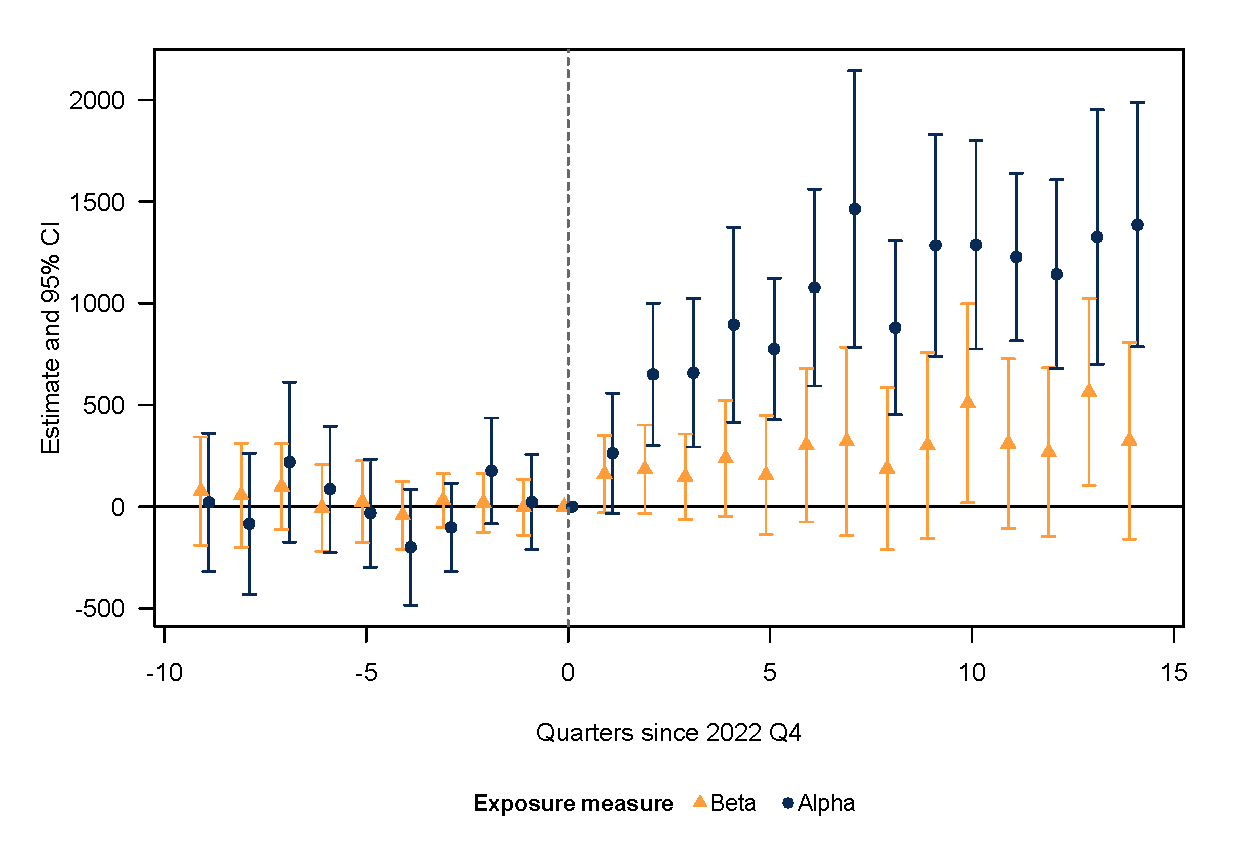
\includegraphics[width=\textwidth]{Figures/es_wage_imp_human.eps}
    \caption{Monthly earnings Human}
    \label{fig:es_wage_imp_human}
  \end{subfigure}

  \medskip

  \begin{subfigure}[b]{0.7\textwidth}
    \centering
    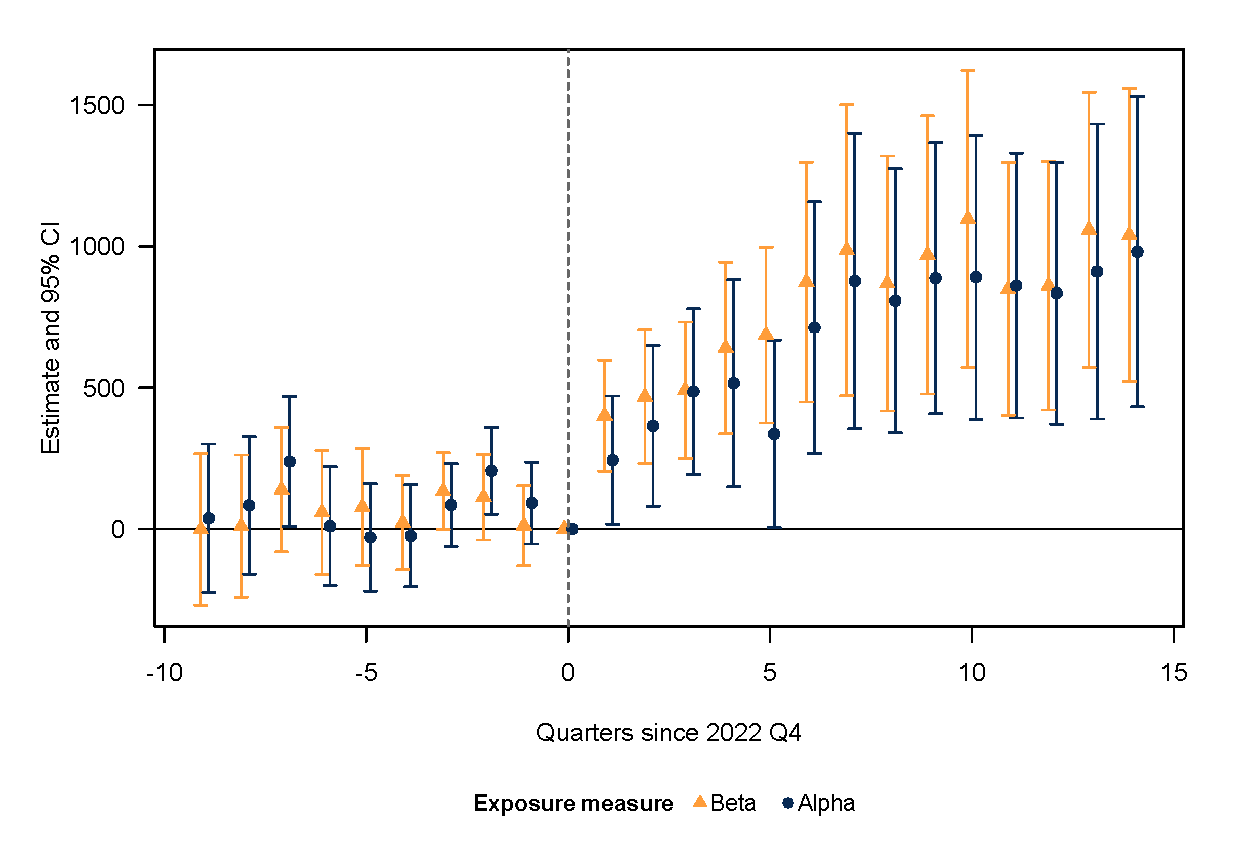
\includegraphics[width=\textwidth]{Figures/es_wage_imp_gpt.eps}
    \caption{Monthly earnings GPT-4o}
    \label{fig:es_wage_imp_gpt}
  \end{subfigure}

  \medskip

  \begin{minipage}{\textwidth}
    \small
    \textit{Note:} The figure shows the main results from my event study analysis (see \cref{ES}). Both panels show the effect on the average monthly earnings of the treated occupations relative to the control occupations over time. Panel (a) uses the human exposure measure, while panel (b) uses the GPT-4o exposure measure. Monthly earnings include observed and imputed values (PMM).
  \end{minipage}
\end{figure}

\begin{figure}[H]
  \centering
  \caption{Impact of ChatGPT's release on the number of workers}
  \label{fig:es_log_emp}

  \begin{subfigure}[b]{0.7\textwidth}
    \centering
    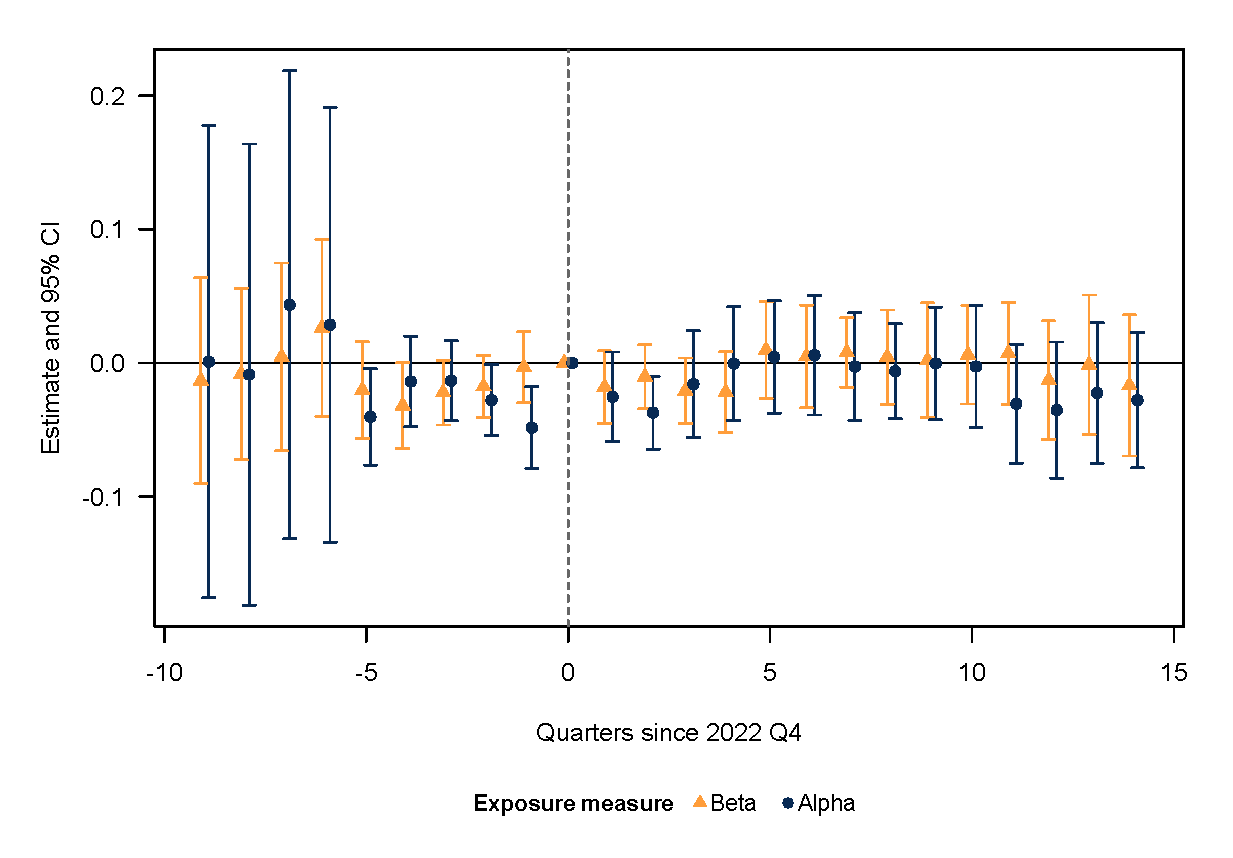
\includegraphics[width=\textwidth]{Figures/es_log_emp_human.eps}
    \caption{Number of workers Human}
    \label{fig:es_log_emp_human}
  \end{subfigure}

  \medskip

  \begin{subfigure}[b]{0.7\textwidth}
    \centering
    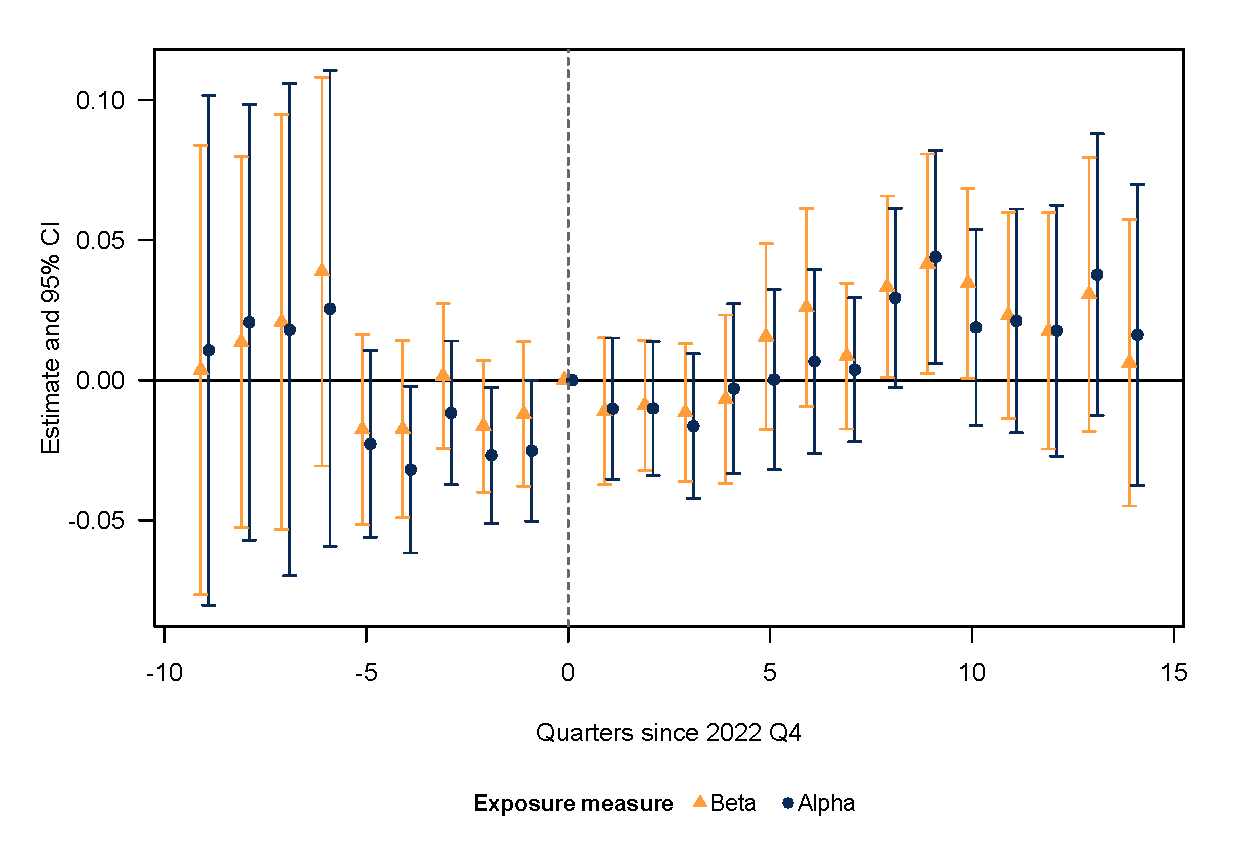
\includegraphics[width=\textwidth]{Figures/es_log_emp_gpt.eps}
    \caption{Number of workers GPT-4o}
    \label{fig:es_log_emp_gpt}
  \end{subfigure}

  \medskip

  \begin{minipage}{\textwidth}
    \small
    \textit{Note:} The figure shows the main results from my event study analysis (see \cref{ES}). Both panels show the effect on the logarithm of the average number of workers of the treated occupations relative to the control occupations over time. Panel (a) uses the human exposure measure, while panel (b) uses the GPT-4o exposure measure.
  \end{minipage}
\end{figure}

\begin{figure}[H]
  \centering
  \caption{Impact of ChatGPT's release on the number of informal workers}
  \label{fig:es_log_informal}

  \begin{subfigure}[b]{0.7\textwidth}
    \centering
    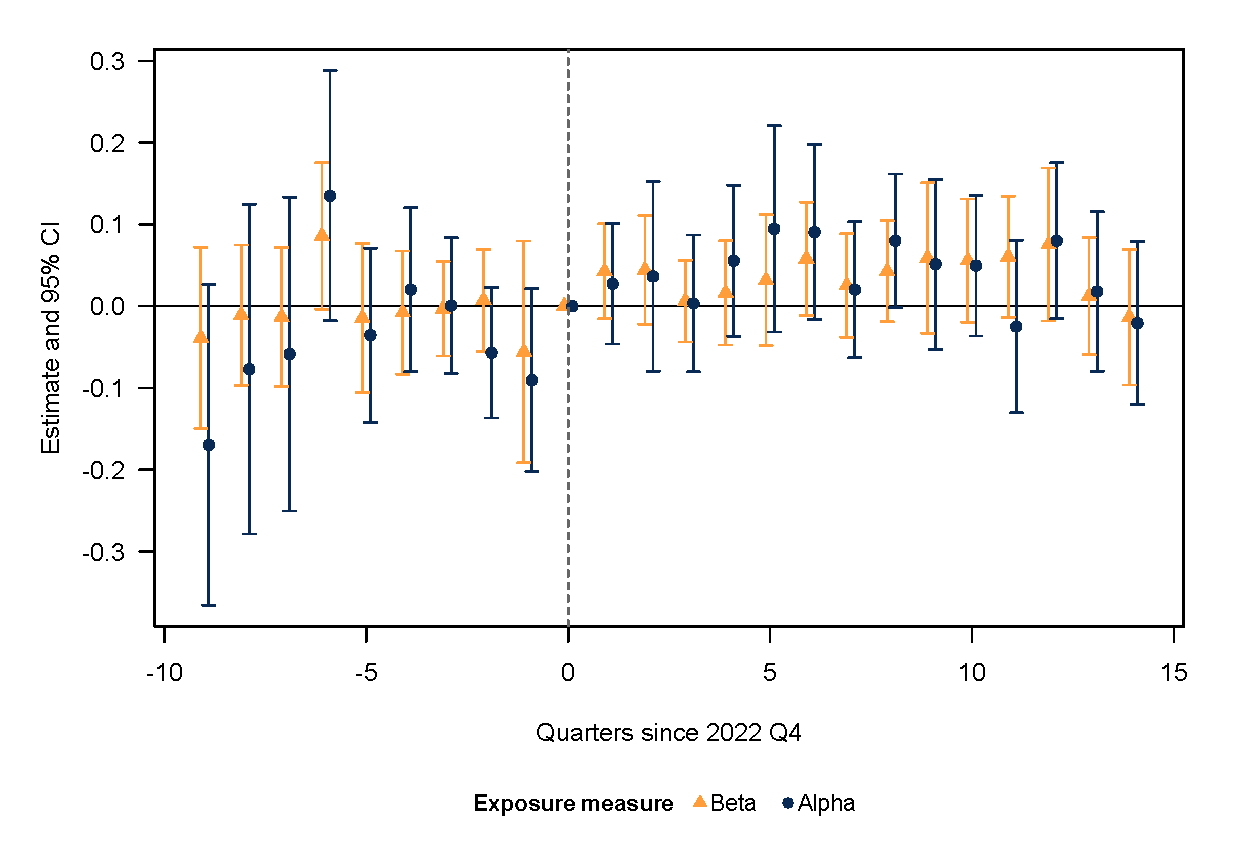
\includegraphics[width=\textwidth]{Figures/es_log_informal_human.eps}
    \caption{Number of informal workers Human}
    \label{fig:es_log_informal_human}
  \end{subfigure}

  \medskip

  \begin{subfigure}[b]{0.7\textwidth}
    \centering
    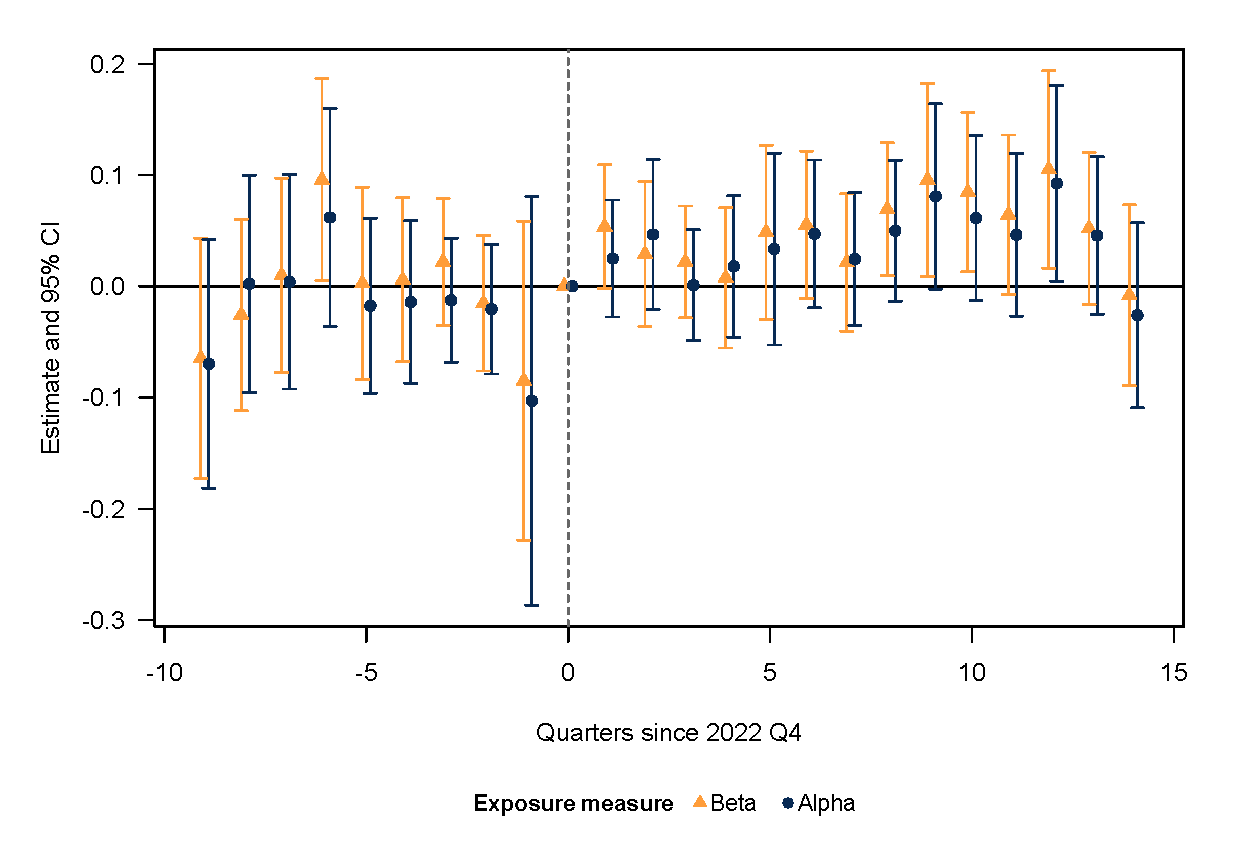
\includegraphics[width=\textwidth]{Figures/es_log_informal_gpt.eps}
    \caption{Number of informal workers GPT-4o}
    \label{fig:es_log_informal_gpt}
  \end{subfigure}

  \medskip

  \begin{minipage}{\textwidth}
    \small
    \textit{Note:} The figure shows the main results from my event study analysis (see \cref{ES}). Both panels show the effect on the logarithm of the average number of informal workers of the treated occupations relative to the control occupations over time. Panel (a) uses the human exposure measure, while panel (b) uses the GPT-4o exposure measure.
  \end{minipage}
\end{figure}

\begingroup
\footnotesize
\renewcommand{\arraystretch}{0.9}
\setlength{\tabcolsep}{4pt}
\begin{longtable}{lcccc}
  \caption{\label{tab:es_wage_imp} Monthly earnings (MXN): event study estimates (ref. = 2022 Q4)}                             \\
  \toprule
                                  & \multicolumn{4}{c}{monthly earnings}                                                       \\
                                  & Human Beta                           & Human Alpha     & GPT-4o Beta     & GPT-4o Alpha    \\
                                  & (1)                                  & (2)             & (3)             & (4)             \\
  \midrule
  \endfirsthead
  \multicolumn{5}{l}{\textit{Table \thetable\ (continued)}}                                                                    \\
  \toprule
                                  & \multicolumn{4}{c}{wage\_imp}                                                              \\
                                  & Human Beta                           & Human Alpha     & GPT-4o Beta     & GPT-4o Alpha    \\
                                  & (1)                                  & (2)             & (3)             & (4)             \\
  \midrule
  \endhead
  \midrule
  \multicolumn{5}{r}{\textit{Continued on next page}}                                                                          \\
  \endfoot
  \bottomrule
  \endlastfoot
  Treated $\times$ Quarter $=$ -9 & 76.7                                 & 20.9            & -1.84           & 38.0            \\
                                  & (135.3)                              & (173.0)         & (136.2)         & (133.7)         \\
  Treated $\times$ Quarter $=$ -8 & 56.0                                 & -84.2           & 9.86            & 83.7            \\
                                  & (129.7)                              & (176.5)         & (128.2)         & (123.7)         \\
  Treated $\times$ Quarter $=$ -7 & 98.4                                 & 219.1           & 139.0           & 238.7$^{**}$    \\
                                  & (107.0)                              & (200.1)         & (111.9)         & (116.9)         \\
  Treated $\times$ Quarter $=$ -6 & -5.91                                & 86.0            & 58.5            & 9.76            \\
                                  & (109.0)                              & (157.8)         & (111.2)         & (107.1)         \\
  Treated $\times$ Quarter $=$ -5 & 23.7                                 & -32.1           & 77.6            & -29.9           \\
                                  & (102.4)                              & (135.1)         & (105.4)         & (96.6)          \\
  Treated $\times$ Quarter $=$ -4 & -42.7                                & -199.2          & 22.6            & -24.3           \\
                                  & (84.6)                               & (145.0)         & (84.7)          & (91.9)          \\
  Treated $\times$ Quarter $=$ -3 & 30.2                                 & -102.0          & 133.5$^{*}$     & 84.7            \\
                                  & (66.8)                               & (110.2)         & (69.1)          & (74.7)          \\
  Treated $\times$ Quarter $=$ -2 & 19.3                                 & 175.7           & 112.4           & 206.1$^{***}$   \\
                                  & (73.7)                               & (132.4)         & (76.8)          & (78.1)          \\
  Treated $\times$ Quarter $=$ -1 & -3.22                                & 22.8            & 11.7            & 91.9            \\
                                  & (70.2)                               & (118.7)         & (72.0)          & (73.7)          \\
  Treated $\times$ Quarter $=$ 1  & 160.1$^{*}$                          & 262.3$^{*}$     & 400.9$^{***}$   & 243.7$^{**}$    \\
                                  & (96.9)                               & (150.4)         & (99.9)          & (115.4)         \\
  Treated $\times$ Quarter $=$ 2  & 184.0$^{*}$                          & 650.5$^{***}$   & 468.1$^{***}$   & 365.3$^{**}$    \\
                                  & (110.7)                              & (178.1)         & (120.5)         & (144.6)         \\
  Treated $\times$ Quarter $=$ 3  & 146.9                                & 658.2$^{***}$   & 491.4$^{***}$   & 486.3$^{***}$   \\
                                  & (106.9)                              & (185.7)         & (122.8)         & (149.0)         \\
  Treated $\times$ Quarter $=$ 4  & 236.3                                & 894.6$^{***}$   & 640.4$^{***}$   & 515.9$^{***}$   \\
                                  & (144.9)                              & (244.1)         & (154.4)         & (186.4)         \\
  Treated $\times$ Quarter $=$ 5  & 155.4                                & 774.8$^{***}$   & 686.2$^{***}$   & 336.2$^{**}$    \\
                                  & (148.1)                              & (177.2)         & (158.2)         & (168.6)         \\
  Treated $\times$ Quarter $=$ 6  & 302.1                                & 1,077.0$^{***}$ & 873.6$^{***}$   & 712.7$^{***}$   \\
                                  & (192.2)                              & (246.1)         & (215.8)         & (226.5)         \\
  Treated $\times$ Quarter $=$ 7  & 319.9                                & 1,463.4$^{***}$ & 986.3$^{***}$   & 877.8$^{***}$   \\
                                  & (235.7)                              & (345.9)         & (261.7)         & (265.9)         \\
  Treated $\times$ Quarter $=$ 8  & 186.6                                & 879.4$^{***}$   & 868.6$^{***}$   & 807.5$^{***}$   \\
                                  & (203.0)                              & (217.3)         & (229.5)         & (237.8)         \\
  Treated $\times$ Quarter $=$ 9  & 301.3                                & 1,284.2$^{***}$ & 969.8$^{***}$   & 887.3$^{***}$   \\
                                  & (232.9)                              & (277.2)         & (250.4)         & (244.0)         \\
  Treated $\times$ Quarter $=$ 10 & 508.3$^{**}$                         & 1,287.4$^{***}$ & 1,097.0$^{***}$ & 891.0$^{***}$   \\
                                  & (248.8)                              & (260.5)         & (267.0)         & (255.5)         \\
  Treated $\times$ Quarter $=$ 11 & 309.5                                & 1,227.3$^{***}$ & 849.4$^{***}$   & 861.5$^{***}$   \\
                                  & (212.2)                              & (209.8)         & (227.5)         & (238.4)         \\
  Treated $\times$ Quarter $=$ 12 & 267.9                                & 1,142.9$^{***}$ & 860.6$^{***}$   & 834.6$^{***}$   \\
                                  & (210.9)                              & (236.1)         & (223.5)         & (235.9)         \\
  Treated $\times$ Quarter $=$ 13 & 564.0$^{**}$                         & 1,325.9$^{***}$ & 1,058.6$^{***}$ & 911.2$^{***}$   \\
                                  & (233.9)                              & (318.4)         & (247.8)         & (265.5)         \\
  Treated $\times$ Quarter $=$ 14 & 324.2                                & 1,385.9$^{***}$ & 1,040.3$^{***}$ & 981.3$^{***}$   \\
                                  & (246.2)                              & (305.3)         & (263.4)         & (279.2)         \\
  female                          & -1,123.5$^{**}$                      & -1,184.2$^{**}$ & -1,237.5$^{**}$ & -1,278.9$^{**}$ \\
                                  & (531.2)                              & (493.7)         & (529.3)         & (517.6)         \\
  anios\_esc                      & 160.8$^{***}$                        & 187.1$^{***}$   & 174.6$^{***}$   & 173.4$^{***}$   \\
                                  & (38.0)                               & (38.5)          & (39.5)          & (38.2)          \\
  eda                             & 10.3                                 & 18.0            & 15.6            & 11.6            \\
                                  & (19.3)                               & (18.7)          & (18.2)          & (18.8)          \\
  \\
  Observations                    & 10,126                               & 10,126          & 10,126          & 10,126          \\
  R$^2$                           & 0.94962                              & 0.95125         & 0.95160         & 0.95092         \\
  \\
  occupation fixed effects        & $\checkmark$                         & $\checkmark$    & $\checkmark$    & $\checkmark$    \\
  period\_q fixed effects         & $\checkmark$                         & $\checkmark$    & $\checkmark$    & $\checkmark$    \\
\end{longtable}
\vspace{-1.5em}
\textit{Note: } Standard errors clustered by occupation. Occupation and quarter fixed effects included, weighted by number of workers per occupation
\endgroup

\newpage

\begingroup
\footnotesize
\renewcommand{\arraystretch}{0.9}
\setlength{\tabcolsep}{4pt}
\begin{longtable}{lcccc}
  \caption{\label{tab:es_log_emp} Log number of workers: event study estimates (ref. = 2022 Q4)}                              \\
  \toprule
                                  & \multicolumn{4}{c}{log number of workers}                                                 \\
                                  & Human Beta                                & Human Alpha    & GPT-4o Beta  & GPT-4o Alpha  \\
                                  & (1)                                       & (2)            & (3)          & (4)           \\
  \midrule
  \endfirsthead
  \multicolumn{5}{l}{\textit{Table \thetable\ (continued)}}                                                                   \\
  \toprule
                                  & \multicolumn{4}{c}{log\_emp}                                                              \\
                                  & Human Beta                                & Human Alpha    & GPT-4o Beta  & GPT-4o Alpha  \\
                                  & (1)                                       & (2)            & (3)          & (4)           \\
  \midrule
  \endhead
  \midrule
  \multicolumn{5}{r}{\textit{Continued on next page}}                                                                         \\
  \endfoot
  \bottomrule
  \endlastfoot
  Treated $\times$ Quarter $=$ -9 & -0.013                                    & 0.0009         & 0.004        & 0.011         \\
                                  & (0.039)                                   & (0.090)        & (0.041)      & (0.046)       \\
  Treated $\times$ Quarter $=$ -8 & -0.008                                    & -0.009         & 0.013        & 0.021         \\
                                  & (0.033)                                   & (0.088)        & (0.034)      & (0.040)       \\
  Treated $\times$ Quarter $=$ -7 & 0.004                                     & 0.044          & 0.021        & 0.018         \\
                                  & (0.036)                                   & (0.089)        & (0.038)      & (0.045)       \\
  Treated $\times$ Quarter $=$ -6 & 0.026                                     & 0.029          & 0.039        & 0.025         \\
                                  & (0.034)                                   & (0.083)        & (0.035)      & (0.043)       \\
  Treated $\times$ Quarter $=$ -5 & -0.020                                    & -0.040$^{**}$  & -0.018       & -0.023        \\
                                  & (0.018)                                   & (0.018)        & (0.017)      & (0.017)       \\
  Treated $\times$ Quarter $=$ -4 & -0.032$^{*}$                              & -0.014         & -0.017       & -0.032$^{**}$ \\
                                  & (0.016)                                   & (0.017)        & (0.016)      & (0.015)       \\
  Treated $\times$ Quarter $=$ -3 & -0.022$^{*}$                              & -0.013         & 0.002        & -0.012        \\
                                  & (0.012)                                   & (0.015)        & (0.013)      & (0.013)       \\
  Treated $\times$ Quarter $=$ -2 & -0.018                                    & -0.028$^{**}$  & -0.016       & -0.027$^{**}$ \\
                                  & (0.012)                                   & (0.013)        & (0.012)      & (0.012)       \\
  Treated $\times$ Quarter $=$ -1 & -0.003                                    & -0.048$^{***}$ & -0.012       & -0.025$^{*}$  \\
                                  & (0.013)                                   & (0.015)        & (0.013)      & (0.013)       \\
  Treated $\times$ Quarter $=$ 1  & -0.018                                    & -0.025         & -0.011       & -0.010        \\
                                  & (0.014)                                   & (0.017)        & (0.013)      & (0.013)       \\
  Treated $\times$ Quarter $=$ 2  & -0.010                                    & -0.037$^{***}$ & -0.009       & -0.010        \\
                                  & (0.012)                                   & (0.014)        & (0.012)      & (0.012)       \\
  Treated $\times$ Quarter $=$ 3  & -0.021$^{*}$                              & -0.016         & -0.012       & -0.016        \\
                                  & (0.012)                                   & (0.020)        & (0.012)      & (0.013)       \\
  Treated $\times$ Quarter $=$ 4  & -0.022                                    & -0.0005        & -0.007       & -0.003        \\
                                  & (0.015)                                   & (0.022)        & (0.015)      & (0.015)       \\
  Treated $\times$ Quarter $=$ 5  & 0.010                                     & 0.004          & 0.015        & 0.0002        \\
                                  & (0.018)                                   & (0.021)        & (0.017)      & (0.016)       \\
  Treated $\times$ Quarter $=$ 6  & 0.005                                     & 0.006          & 0.026        & 0.007         \\
                                  & (0.020)                                   & (0.023)        & (0.018)      & (0.017)       \\
  Treated $\times$ Quarter $=$ 7  & 0.008                                     & -0.003         & 0.009        & 0.004         \\
                                  & (0.013)                                   & (0.020)        & (0.013)      & (0.013)       \\
  Treated $\times$ Quarter $=$ 8  & 0.004                                     & -0.006         & 0.033$^{**}$ & 0.029$^{*}$   \\
                                  & (0.018)                                   & (0.018)        & (0.016)      & (0.016)       \\
  Treated $\times$ Quarter $=$ 9  & 0.002                                     & -0.0004        & 0.042$^{**}$ & 0.044$^{**}$  \\
                                  & (0.022)                                   & (0.021)        & (0.020)      & (0.019)       \\
  Treated $\times$ Quarter $=$ 10 & 0.006                                     & -0.003         & 0.035$^{**}$ & 0.019         \\
                                  & (0.019)                                   & (0.023)        & (0.017)      & (0.018)       \\
  Treated $\times$ Quarter $=$ 11 & 0.007                                     & -0.030         & 0.023        & 0.021         \\
                                  & (0.019)                                   & (0.023)        & (0.019)      & (0.020)       \\
  Treated $\times$ Quarter $=$ 12 & -0.013                                    & -0.035         & 0.018        & 0.018         \\
                                  & (0.023)                                   & (0.026)        & (0.021)      & (0.023)       \\
  Treated $\times$ Quarter $=$ 13 & -0.001                                    & -0.023         & 0.031        & 0.038         \\
                                  & (0.026)                                   & (0.027)        & (0.025)      & (0.026)       \\
  Treated $\times$ Quarter $=$ 14 & -0.017                                    & -0.028         & 0.006        & 0.016         \\
                                  & (0.027)                                   & (0.026)        & (0.026)      & (0.027)       \\
  female                          & 0.107                                     & 0.106          & 0.103        & 0.100         \\
                                  & (0.075)                                   & (0.077)        & (0.074)      & (0.074)       \\
  anios\_esc                      & 0.002                                     & 0.001          & 0.002        & 0.003         \\
                                  & (0.008)                                   & (0.006)        & (0.008)      & (0.008)       \\
  eda                             & -0.011$^{**}$                             & -0.011$^{**}$  & -0.011$^{*}$ & -0.011$^{**}$ \\
                                  & (0.005)                                   & (0.005)        & (0.005)      & (0.005)       \\
  \\
  Observations                    & 10,128                                    & 10,128         & 10,128       & 10,128        \\
  R$^2$                           & 0.99153                                   & 0.99153        & 0.99155      & 0.99155       \\
  \\
  occupation fixed effects        & $\checkmark$                              & $\checkmark$   & $\checkmark$ & $\checkmark$  \\
  period\_q fixed effects         & $\checkmark$                              & $\checkmark$   & $\checkmark$ & $\checkmark$  \\
\end{longtable}
\vspace{-1.5em}
\textit{Notes:} Standard errors clustered by occupation. Occupation and quarter fixed effects included, weighted by number of workers per occupation
\endgroup

\newpage

\begingroup
\footnotesize
\renewcommand{\arraystretch}{0.9}
\setlength{\tabcolsep}{4pt}
\begin{longtable}{lcccc}
  \caption{\label{tab:es_log_informal} Log number of informal workers: event study estimates (ref. = 2022 Q4)}                            \\
  \toprule
                                  & \multicolumn{4}{c}{log number of informal workers}                                                    \\
                                  & Human Beta                                         & Human Alpha    & GPT-4o Beta    & GPT-4o Alpha   \\
                                  & (1)                                                & (2)            & (3)            & (4)            \\
  \midrule
  \endfirsthead
  \multicolumn{5}{l}{\textit{Table \thetable\ (continued)}}                                                                               \\
  \toprule
                                  & \multicolumn{4}{c}{log\_informal}                                                                     \\
                                  & Human Beta                                         & Human Alpha    & GPT-4o Beta    & GPT-4o Alpha   \\
                                  & (1)                                                & (2)            & (3)            & (4)            \\
  \midrule
  \endhead
  \midrule
  \multicolumn{5}{r}{\textit{Continued on next page}}                                                                                     \\
  \endfoot
  \bottomrule
  \endlastfoot
  Treated $\times$ Quarter $=$ -9 & -0.039                                             & -0.170$^{*}$   & -0.065         & -0.070         \\
                                  & (0.056)                                            & (0.100)        & (0.055)        & (0.057)        \\
  Treated $\times$ Quarter $=$ -8 & -0.011                                             & -0.077         & -0.026         & 0.002          \\
                                  & (0.044)                                            & (0.103)        & (0.044)        & (0.050)        \\
  Treated $\times$ Quarter $=$ -7 & -0.013                                             & -0.059         & 0.010          & 0.004          \\
                                  & (0.043)                                            & (0.098)        & (0.044)        & (0.049)        \\
  Treated $\times$ Quarter $=$ -6 & 0.086$^{*}$                                        & 0.135$^{*}$    & 0.096$^{**}$   & 0.062          \\
                                  & (0.045)                                            & (0.078)        & (0.046)        & (0.050)        \\
  Treated $\times$ Quarter $=$ -5 & -0.014                                             & -0.035         & 0.003          & -0.018         \\
                                  & (0.046)                                            & (0.054)        & (0.044)        & (0.040)        \\
  Treated $\times$ Quarter $=$ -4 & -0.008                                             & 0.020          & 0.006          & -0.014         \\
                                  & (0.038)                                            & (0.051)        & (0.037)        & (0.037)        \\
  Treated $\times$ Quarter $=$ -3 & -0.003                                             & 0.0006         & 0.022          & -0.012         \\
                                  & (0.029)                                            & (0.042)        & (0.029)        & (0.028)        \\
  Treated $\times$ Quarter $=$ -2 & 0.007                                              & -0.057         & -0.015         & -0.020         \\
                                  & (0.032)                                            & (0.041)        & (0.031)        & (0.030)        \\
  Treated $\times$ Quarter $=$ -1 & -0.056                                             & -0.090         & -0.085         & -0.103         \\
                                  & (0.069)                                            & (0.057)        & (0.073)        & (0.093)        \\
  Treated $\times$ Quarter $=$ 1  & 0.043                                              & 0.028          & 0.053$^{*}$    & 0.025          \\
                                  & (0.029)                                            & (0.037)        & (0.028)        & (0.027)        \\
  Treated $\times$ Quarter $=$ 2  & 0.044                                              & 0.036          & 0.029          & 0.046          \\
                                  & (0.034)                                            & (0.059)        & (0.033)        & (0.034)        \\
  Treated $\times$ Quarter $=$ 3  & 0.006                                              & 0.003          & 0.022          & 0.001          \\
                                  & (0.025)                                            & (0.043)        & (0.026)        & (0.025)        \\
  Treated $\times$ Quarter $=$ 4  & 0.016                                              & 0.056          & 0.008          & 0.018          \\
                                  & (0.032)                                            & (0.047)        & (0.032)        & (0.032)        \\
  Treated $\times$ Quarter $=$ 5  & 0.032                                              & 0.095          & 0.048          & 0.033          \\
                                  & (0.041)                                            & (0.064)        & (0.040)        & (0.044)        \\
  Treated $\times$ Quarter $=$ 6  & 0.058                                              & 0.091$^{*}$    & 0.055          & 0.047          \\
                                  & (0.035)                                            & (0.054)        & (0.034)        & (0.034)        \\
  Treated $\times$ Quarter $=$ 7  & 0.025                                              & 0.020          & 0.021          & 0.024          \\
                                  & (0.032)                                            & (0.042)        & (0.032)        & (0.030)        \\
  Treated $\times$ Quarter $=$ 8  & 0.043                                              & 0.080$^{*}$    & 0.069$^{**}$   & 0.050          \\
                                  & (0.031)                                            & (0.042)        & (0.030)        & (0.032)        \\
  Treated $\times$ Quarter $=$ 9  & 0.059                                              & 0.051          & 0.096$^{**}$   & 0.081$^{*}$    \\
                                  & (0.047)                                            & (0.053)        & (0.044)        & (0.042)        \\
  Treated $\times$ Quarter $=$ 10 & 0.056                                              & 0.050          & 0.085$^{**}$   & 0.061          \\
                                  & (0.038)                                            & (0.044)        & (0.036)        & (0.038)        \\
  Treated $\times$ Quarter $=$ 11 & 0.060                                              & -0.025         & 0.064$^{*}$    & 0.046          \\
                                  & (0.038)                                            & (0.054)        & (0.036)        & (0.037)        \\
  Treated $\times$ Quarter $=$ 12 & 0.075                                              & 0.080          & 0.105$^{**}$   & 0.092$^{**}$   \\
                                  & (0.048)                                            & (0.049)        & (0.045)        & (0.045)        \\
  Treated $\times$ Quarter $=$ 13 & 0.012                                              & 0.018          & 0.052          & 0.046          \\
                                  & (0.037)                                            & (0.050)        & (0.035)        & (0.036)        \\
  Treated $\times$ Quarter $=$ 14 & -0.013                                             & -0.021         & -0.008         & -0.026         \\
                                  & (0.042)                                            & (0.051)        & (0.041)        & (0.042)        \\
  female                          & 0.256$^{**}$                                       & 0.262$^{**}$   & 0.251$^{**}$   & 0.246$^{**}$   \\
                                  & (0.118)                                            & (0.118)        & (0.117)        & (0.117)        \\
  anios\_esc                      & -0.024                                             & -0.023         & -0.024         & -0.024         \\
                                  & (0.016)                                            & (0.016)        & (0.016)        & (0.016)        \\
  eda                             & -0.018$^{***}$                                     & -0.018$^{***}$ & -0.018$^{***}$ & -0.018$^{***}$ \\
                                  & (0.005)                                            & (0.005)        & (0.005)        & (0.005)        \\
  \\
  Observations                    & 10,128                                             & 10,128         & 10,128         & 10,128         \\
  R$^2$                           & 0.97502                                            & 0.97506        & 0.97508        & 0.97505        \\
  \\
  occupation fixed effects        & $\checkmark$                                       & $\checkmark$   & $\checkmark$   & $\checkmark$   \\
  period\_q fixed effects         & $\checkmark$                                       & $\checkmark$   & $\checkmark$   & $\checkmark$   \\
\end{longtable}
\vspace{-1.5em}
\textit{Notes:} Standard errors clustered by occupation. Occupation and quarter fixed effects included, weighted by number of workers per occupation
\endgroup

\begin{figure}[H]
  \centering
  \caption{Placebo tests}
  \label{fig:placebo}

  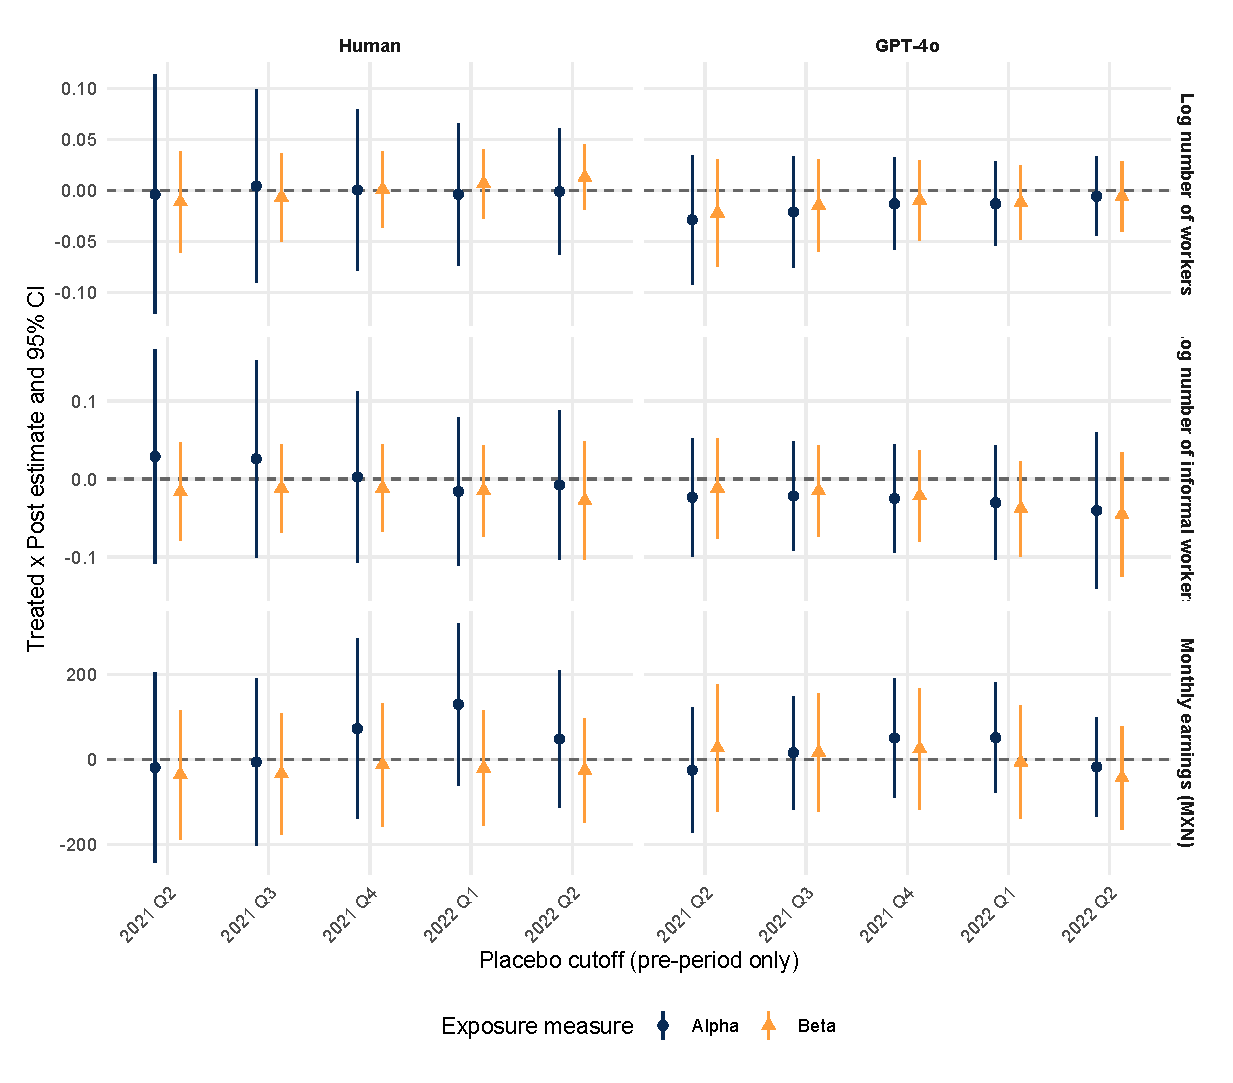
\includegraphics[width=\textwidth]{Figures/placebo_time.eps}

  \begin{minipage}{\textwidth}
    \small
    \textit{Note:} The figure shows placebo tests for every period before treatment in 2022Q4 and measures $\alpha$ and $\beta$. Each estimate plots $\text{Post}_{t} \times \text{ExposureGPT}_j$ for monthly earnings, number of informal workers and number of workers.
  \end{minipage}
\end{figure}
\newpage
\bibliographystyle{chicago}
\bibliography{Bib/Literature}
\newpage
\listoffigures
\newpage


\end{document}
